\documentclass[nonblindrev,copyedit]{informs1}

\usepackage{natbib}
\bibpunct[, ]{(}{)}{,}{a}{}{,}
\def\bibfont{\small}
\def\bibsep{1pt plus .3ex}
\def\bibhang{24pt}
\def\newblock{\ }
\def\BIBand{and}

\usepackage{amsmath,amssymb,mathtools}
\usepackage{mathpazo}
\usepackage{graphicx}
\usepackage[justification=centering]{caption}
\usepackage{subcaption}
\usepackage{hyperref}

\TheoremsNumberedThrough

\begin{document}
\RUNAUTHOR{Jiang et al. (2026)}
\RUNTITLE{Online Appendix: Dynamic Competition with C2C}

\setcounter{page}{1}
\numberwithin{equation}{section}
\numberwithin{lemma}{section}
\numberwithin{proposition}{section}
\numberwithin{figure}{section}

\begin{APPENDICES}

\begin{center}
{\large\bfseries Online Appendix to ``Dynamic Competition in Online Retailing: Implications of Customer-to-Customer Interactions"\par}
Zheyu Jiang, Xin Geng, Nan Yang, and Renyu Zhang
\end{center}

\section{Proof of Statements} \label{appdx-proof}

\subsection{Proof of Statements in Section 4}
{\bf Proof of Lemma 1}: In the benchmark scenario, retailer A maximizes its single-period profit in each period $t$:
\begin{eqnarray*} \label{model0:A}
    \max_{y_{A,t}} p_{A,t} \mathbb{E}\left[y_{A,t} \wedge D_{A,t}  \right] - c_A y_{A,t} = (p_{A,t} - c_A )y_{A,t} - p_{A,t} \mathbb{E} \left[y_{A,t} - D_{A,t}  \right]^+,
\end{eqnarray*}
where $D_{A,t} = \alpha_{A,t} X_t + \theta \left[\alpha_{B,t} X_t - y_{B,t} \right]^+$. Retailer A's profit is concave in $y_{A,t}$ and its derivative w.r.t $y_{A,t}$ is $p_{A,t} - c_A - p_{A,t} \mathbf{Prob} \left(D_{A,t} \leq y_{A,t} \right)$, where
\begin{eqnarray} \label{prob0:A}
    \mathbf{Prob} \left(D_{A,t} \leq y_{A,t} \right)
     =  \int_{0}^{y_{B,t}/\alpha_{B,t}} \mathbb{1}_{ \left \{z \leq y_{A,t}/\alpha_{A,t} \right \} } f(z) dz + \int_{y_{B,t}/\alpha_{B,t}}^{+\infty} \mathbb{1}_{ \left \{z \leq \frac{y_{A,t}+\theta y_{B,t}}{\alpha_{A,t}+\theta \alpha_{B,t}}  \right \} } f(z) dz.
\end{eqnarray}
If $y_{A,t}/\alpha_{A,t} \geq y_{B,t}/\alpha_{B,t}$, $\frac{y_{B,t}}{\alpha_{B,t}} \leq \frac{y_{A,t}+\theta y_{B,t}}{\alpha_{A,t}+\theta \alpha_{B,t}}  \leq \frac{y_{A,t}}{\alpha_{A,t}}$ for $\theta \in [0,1]$. Thus, by (\ref{prob0:A}), we have $\mathbf{Prob} \left(D_{A,t} \leq y_{A,t} \right) = F\left(\frac{y_{A,t}+\theta y_{B,t}}{\alpha_{A,t}+\theta \alpha_{B,t}}\right)$. If $y_{A,t}/\alpha_{A,t} < y_{B,t}/\alpha_{B,t}$, $\frac{y_{A,t}}{\alpha_{A,t}} \leq \frac{y_{A,t}+\theta y_{B,t}}{\alpha_{A,t}+\theta \alpha_{B,t}} < \frac{y_{B,t}}{\alpha_{B,t}}$ for $\theta \in [0,1]$. Thus, by (\ref{prob0:A}), we have $\mathbf{Prob} \left(D_{A,t} \leq y_{A,t} \right) = F\left(\frac{y_{A,t}}{\alpha_{A,t}}\right)$. Therefore, the best response of retailer A is
\begin{equation} \label{model0:BRA}
    y^*_{A,t}(y_{B,t}) =  \begin{cases}
        (\alpha_{A,t} + \theta \alpha_{B,t}) \zeta^0_{A,t} - \theta y_{B,t}, &  \text{if $y_{B,t} \leq \alpha_{B,t} \zeta^0_{A,t}$,} \\
        \alpha_{A,t} \zeta^0_{A,t}, &  \text{if $y_{B,t} > \alpha_{B,t} \zeta^0_{A,t}$,}
    \end{cases}
\end{equation}
where $\zeta^0_{A,t} := F^{-1}(1 - \frac{c_A}{p_{A,t}})$. On the other hand, retailer B's problem is as follows:
\begin{eqnarray*} \label{model0:B}
    \max_{y_{B,t}} p_{B,t} \mathbb{E}\left[y_{B,t} \wedge D_{B,t}  \right] - c_B y_{B,t} = (p_{B,t} -c_B)y_{B,t} - p_{B,t} \mathbb{E} \left[y_{B,t} - D_{B,t}  \right]^+,
\end{eqnarray*}
where $D_{B,t} = \alpha_{B,t} X_t + \theta \left[\alpha_{A,t} X_t - y_{A,t} \right]^+$. By analogous arguments, the best response of retailer B is
\begin{equation}  \label{model0:BRB}
    y^*_{B,t}(y_{A,t}) =  \begin{cases}
        (\alpha_{B,t} + \theta \alpha_{A,t}) \zeta^0_{B,t} - \theta y_{A,t}, &  \text{if $y_{A,t} \leq \alpha_{A,t} \zeta^0_{B,t}$,} \\
        \alpha_{B,t} \zeta^0_{B,t}, &  \text{if $y_{A,t} > \alpha_{A,t} \zeta^0_{B,t}$,}
    \end{cases}
\end{equation}
where $\zeta^0_{B,t} := F^{-1}(1 - \frac{c_B}{p_{B,t}})$.

Since $p_{B,t} c_A/c_B \leq p_{A,t}$, we have $\zeta^0_{A,t} \geq \zeta^0_{B,t}$ for $t = 1, 2$. By combining (\ref{model0:BRA}) and (\ref{model0:BRB}), for each period $t$, there exists a unique Nash equilibrium $(y^0_{A,t},y^0_{B,t})$, where $y^0_{A,t} := (\alpha_{A,t} + \theta \alpha_{B,t}) \zeta^0_{A,t} - \theta \alpha_{B,t} \zeta^0_{B,t}$ and $y^0_{B,t} : = \alpha_{B,t} \zeta^0_{B,t}$.

Last, by substituting $y^0_{A,t}$ and $y^0_{B,t}$ into retailers' profit functions, retailers A's and B's equilibrium profits in benchmark scenario are $\pi^{0}_{A,t}$ and $\pi^{0}_{B,t}$, respectively: $\pi^{0}_{A,t} := (p_{A,t}-c_A)y^0_{A,t} - p_{A,t} \mathbb{E}[L^0_{A,t}]$ and $\pi^{0}_{B,t} := (p_{B,t}-c_B)y^0_{B,t} - p_{B,t} \mathbb{E}[L^0_{B,t}]$,
where $L^0_{A,t} := \left[(\alpha_{A,t} + \theta \alpha_{B,t}) \zeta^0_{A,t} - \theta \alpha_{B,t} \zeta^0_{B,t} - \alpha_{A,t} X_t - \theta (\alpha_{B,t} X_t - \alpha_{B,t} \zeta^0_{B,t})^+ \right]^+$ and $L^0_{B,t} := \left[\alpha_{B,t} \zeta^0_{B,t} - \alpha_{B,t} X_t - \theta \left \{\alpha_{A,t} X_t - (\alpha_{A,t} + \theta \alpha_{B,t}) \zeta^0_{A,t} + \theta \alpha_{B,t} \zeta^0_{B,t} \right \}^+ \right]^+$, $t = 1,2$. Furthermore, retailer $i$'s equilibrium sales in each period are $R^{0}_{i,t} := y^0_{i,t} - L^0_{i,t}$, $i = A,B$ and $t = 1,2$. $\qed$

{\bf Proof of Lemma 2}: We first study the subgame in the second period. Given the first-period seed demand $X_1$ and retailers' first-period sales, retailer A maximizes its second-period profit:
\begin{eqnarray}
    & & \max_{y_{A,2}} \mathbb{E}\left[ p_{A,2}(y_{A,2} \wedge D_{A,2}) - c_A y_{A,2}|X_1  \right] \nonumber \\
    & = & \mathbb{E} \left[ (p_{A,2} -c_A)y_{A,2} - p_{A,2} \left(y_{A,2} - \alpha_{A,2} X_2 - \gamma R_{A,1} - \theta \left(\alpha_{B,2} X_2 + \gamma R_{B,1}- y_{B,2} \right)^+ \right )^+  \bigg| X_1  \right] \nonumber \\[4pt]
    & = & \mathbb{E} \left[ (p_{A,2} -c_A)\overline{y}_{A,2} - p_{A,2} \left(\overline{y}_{A,2} - \alpha_{A,2} X_2  - \theta \left(\alpha_{B,2} X_2 - \overline{y}_{B,2} \right)^+ \right )^+ + (p_{A,2} -c_A)\gamma R_{A,1} \bigg| X_1  \right]  \label{models:A2}
\end{eqnarray}
where $D_{A,2} = \alpha_{A,2} X_2 + \gamma R_{A,1} + \theta \left[\alpha_{B,2} X_2 + \gamma R_{B,1} - y_{B,2} \right]^+$, $\overline{y}_{A,2} := y_{A,2} - \gamma R_{A,1}$, and $\overline{y}_{B,2} := y_{B,2} - \gamma R_{B,1}$. Given firm $i$'s first-period sales, $\overline{y}_{i,2}$ is uniquely determined by $y_{i,2}$. Thus, we use $\overline{y}_{A,2}$ and $\overline{y}_{B,2}$ as firm A's and firm B's second-period decision, respectively. Note that the profit function in (\ref{models:A2}) is concave in $\overline{y}_{A,2}$. By analogous arguments in the proof of Lemma 1, retailer A's best response in the second period is:
\begin{equation} \label{models:BRA2}
    \overline{y}^*_{A,2}(\overline{y}_{B,2}) =  \begin{cases}
         (\alpha_{A,2} + \theta \alpha_{B,2}) \zeta^0_{A,2} - \theta \overline{y}_{B,2}, &  \text{if $\overline{y}_{B,2} \leq \alpha_{B,2} \zeta^0_{A,2}$,} \\
         \alpha_{A,2} \zeta^0_{A,2}, &  \text{if $\overline{y}_{B,2} > \alpha_{B,2}  \zeta^0_{A,2}$.}
    \end{cases}
\end{equation}

On the other hand, given $X_1$ and retailers' first-period sales, retailer B maximizes its second-period profit:
\begin{eqnarray}
    & & \max_{y_{B,2}} \mathbb{E}\left[ p_{B,2}(y_{B,2} \wedge D_{B,2}) - c_B y_{B,2}|X_1  \right] \nonumber \\
    & = & \mathbb{E} \left[ (p_{B,2} -c_B)y_{B,2} - p_{B,2} \left(y_{B,2} - \alpha_{B,2} X_2 - \gamma R_{B,1} - \theta \left(\alpha_{A,2} X_2 + \gamma R_{A,1}- y_{A,2} \right)^+ \right )^+  \bigg| X_1  \right] \nonumber \\[4pt]
    & = & \mathbb{E} \left[ (p_{B,2} -c_B)\overline{y}_{B,2} - p_{B,2} \left(\overline{y}_{B,2} - \alpha_{B,2} X_2  - \theta \left(\alpha_{A,2} X_2 - \overline{y}_{A,2} \right)^+ \right )^+ + (p_{B,2} -c_B)\gamma R_{B,1} \bigg| X_1  \right],  \label{models:B2}
\end{eqnarray}
where $D_{B,2} = \alpha_{B,2} X_2 + \gamma R_{B,1} + \theta \left[\alpha_{A,2} X_2 + \gamma R_{A,1} - y_{A,2} \right]^+$. Retailer B's profit function in (\ref{models:B2}) is concave in $\overline{y}_{B,2}$. By analogous arguments in the proof of Lemma 1, retailer B's best response in the second period is:
\begin{equation}  \label{models:BRB2}
    \overline{y}^*_{B,2}(\overline{y}_{A,2}) =  \begin{cases}
        (\alpha_{B,2} + \theta \alpha_{A,2}) \zeta^0_{B,2} - \theta \overline{y}_{A,2}, &  \text{if $\overline{y}_{A,2} \leq \alpha_{A,2} \zeta^0_{B,2}$,} \\
        \alpha_{B,2} \zeta^0_{B,2}, &  \text{if $\overline{y}_{A,2} > \alpha_{A,2} \zeta^0_{B,2}$,}
    \end{cases}
\end{equation}

By combining (\ref{models:BRA2}) and (\ref{models:BRB2}), there exists a unique Nash equilibrium in the second period, $(\overline{y}^S_{A,2},\overline{y}^S_{B,2})$, where $\overline{y}^S_{A,2} = y^0_{A,2}$ and $\overline{y}^S_{B,2} = y^0_{B,2}$. That is, retailers' equilibrium order quantities are $y^S_{A,2} = y^0_{A,2} +\gamma R_{A,1}$ and $y^S_{B,2} = y^0_{B,2} +\gamma R_{B,1}$.
Furthermore, by substituting $\overline{y}^S_{A,2}$ and $\overline{y}^S_{B,2}$ into (\ref{models:A2}) and (\ref{models:B2}), retailer A's second-period profit equals $\pi^{0}_{A,2} + (p_{A,2} -c_A)\gamma \mathbb{E} \left[ R_{A,1} | X_1  \right]$ and retailer B's second period profit equals $\pi^{0}_{B,2} + (p_{B,2} -c_B)\gamma \mathbb{E} \left[ R_{B,1} | X_1  \right]$.
Next, we study two retailers' competition in the first period. Retailer A optimizes its order quantity to maximize its profit in two periods:
\begin{eqnarray}
    & & \max_{y_{A,1}} p_{A,1} \mathbb{E}\left[y_{A,1} \wedge D_{A,1}  \right] - c_A y_{A,1} + \rho (p_{A,2} -c_A)\gamma \mathbb{E} \left[y_{A,1} \wedge D_{A,1}  \right] + \rho \pi^{0}_{A,2} \nonumber \\
    & = & [p_{A,1} -c_A + \rho (p_{A,2} -c_A)\gamma]y_{A,1} - [p_{A,1}+\rho (p_{A,2} -c_A)\gamma] \mathbb{E} \left[y_{A,1} - D_{A,1}  \right]^+ + \rho \pi^{0}_{A,2}, \label{models:A1}
\end{eqnarray}
where $D_{A,1} = \alpha_{A,1} X_1 + \theta \left[\alpha_{B,1} X_1 - y_{B,1} \right]^+$. Note that profit function in (\ref{models:A1}) is concave in $y_{A,1}$ and its derivative w.r.t. $y_{A,1}$ is $p_{A,1} - c_A + \rho \gamma(p_{A,2} - c_A) - [p_{A,1} + \rho \gamma (p_{A,2} - c_A)] \mathbf{Prob} \left(D_{A,1} \leq y_{A,1} \right)$, where $\mathbf{Prob} \left(D_{A,1} \leq y_{A,1} \right)$ follows (\ref{prob0:A}). Thus, by analogous arguments in the proof of Lemma 1, the best response of retailer A is
\begin{equation} \label{models:BRA1}
    y^*_{A,1}(y_{B,1}) =  \begin{cases}
        (\alpha_{A,1} + \theta \alpha_{B,1}) \zeta^S_{A,1} - \theta y_{B,1}, &  \text{if $y_{B,1} \leq \alpha_{B,1} \zeta^S_{A,1}$,} \\
        \alpha_{A,1} \zeta^S_{A,1}, &  \text{if $y_{B,1} > \alpha_{B,1} \zeta^S_{A,1}$,}
    \end{cases}
\end{equation}
where $\zeta^S_{A,1} := F^{-1}(1 - \frac{c_A}{p_{A,1} + \rho \gamma (p_{A,2}-c_A)})$. On the other hand, retailer B optimizes its order quantity to maximize its total profit in two periods:
\begin{eqnarray}
    & & \max_{y_{B,1}}  p_{B,1} \mathbb{E}\left[y_{B,1} \wedge D_{B,1}  \right] - c_B y_{B,1} + \rho (p_{B,2} -c_B)\gamma \mathbb{E} \left[y_{B,1} \wedge D_{B,1}  \right] + \rho \pi^{0}_{B,2} \nonumber \\
    & = & [p_{B,1} -c_B + \rho (p_{B,2} -c_B)\gamma]y_{B,1} - [p_{B,1}+\rho (p_{B,2} -c_B)\gamma] \mathbb{E} \left[y_{B,1} - D_{B,1}  \right]^+ + \rho \pi^{0}_{B,2}, \label{models:B1}
\end{eqnarray}
where $D_{B,1} = \alpha_{B,1} X_1 + \theta \left[\alpha_{A,1} X_1 - y_{A,1} \right]^+$. Note that the profit function in (\ref{models:B1}) is concave in $y_{B,1}$. By analogous arguments, retailer B's best response is
\begin{equation}  \label{models:BRB1}
    y^*_{B,1}(y_{A,1}) =  \begin{cases}
        (\alpha_{B,1} + \theta \alpha_{A,1}) \zeta^S_{B,1} - \theta y_{A,1}, &  \text{if $y_{A,1} \leq \alpha_{A,1} \zeta^S_{B,1}$,} \\
        \alpha_{B,1} \zeta^S_{B,1}, &  \text{if $y_{A,1} > \alpha_{A,1} \zeta^S_{B,1}$,}
    \end{cases}
\end{equation}
where $\zeta^S_{B,1} := F^{-1}(1 - \frac{c_B}{p_{B,1}+\rho \gamma (p_{B,2}-c_B)})$. Note that $\zeta^S_{i,1} > \zeta^0_{i,1}$ for $\gamma > 0$, when $\rho >0$ and $p_{i,t}>c_i$.

Since $p_{B,t} c_A/c_B \leq p_{A,t}$, $t= 1,2$, we have $\frac{c_A}{p_{A,1}+\rho \gamma (p_{A,2}-c_A)} \leq \frac{c_B}{p_{B,1}+\rho \gamma (p_{B,2}-c_B)}$ and thus $\zeta^S_{A,1} \geq \zeta^S_{B,1}$. By combining (\ref{models:BRA1}) and (\ref{models:BRB1}), there exists a unique Nash equilibrium $(y^S_{A,1},y^S_{B,1})$, where $y^S_{A,1} = (\alpha_{A,1} + \theta \alpha_{B,1}) \zeta^S_{A,1} - \theta \alpha_{B,1} \zeta^S_{B,1}$, $y^S_{B,1} = \alpha_{B,1} \zeta^S_{B,1}$, and $\zeta^S_{i,1} : =F^{-1}(1 - \frac{c_i}{p_{i,1}+\rho \gamma (p_{i,2}-c_i)})$, $i = A, B$.

Last, by substituting $y^S_{A,1}$ and $y^S_{B,1}$ into (\ref{models:A1}) and (\ref{models:B1}), we have retailers' equilibrium profits as follows: $\Pi^{S}_{A} = [p_{A,1} -c_A + \rho (p_{A,2} -c_A)\gamma] y^S_{A,1} - [p_{A,1}+\rho (p_{A,2} -c_A)\gamma] \mathbb{E} [L^S_{A,1}] + \rho \pi^{0}_{A,2} $ and $\Pi^{S}_{B} = [p_{B,1} -c_B + \rho (p_{B,2} -c_B)\gamma] y^S_{B,1} - [p_{B,1}+\rho (p_{B,2} -c_B)\gamma] \mathbb{E}[L^S_{B,1}] + \rho \pi^{0}_{B,2}$, where $L^S_{A,1} :=  [(\alpha_{A,1}+\theta \alpha_{B,1})\zeta^S_{A,1} - \theta \alpha_{B,1} \zeta^S_{B,1} - \alpha_{A,1} X_1 - \theta (\alpha_{B,1} X_1 - \alpha_{B,1} \zeta^S_{B,1})^+ ]^+ $ and $L^S_{B,1} := [\alpha_{B,1} \zeta^S_{B,1} - \alpha_{B,1} X_1 - \theta \{\alpha_{A,1} X_1 - (\alpha_{A,1} + \theta \alpha_{B,1})\zeta^S_{A,1} +\theta \alpha_{B,1} \zeta^S_{B,1} \}^+ ]^+$. Furthermore, retailers' equilibrium first-period sales are $R^{S}_{A,1} := y^S_{A,1} - L^S_{A,1}$ and $R^{S}_{B,1} := y^S_{B,1} - L^S_{B,1}$ and second-period order quantities are $y^{S}_{A,2} = y_{A,2}^0 + \gamma R_{A,1}^S$ and $y^{S}_{B,2} = y_{B,2}^0 +  \gamma R_{B,1}^S$. $\qed$

{\bf Proof of Lemma 3}: We first study the subgame in the second period. Retailers' demand is $D_{A,2}= \alpha_{A,2} X_2 + \alpha_{A,2} \gamma R_{1} + \theta \left[\alpha_{B,2} X_2 + \alpha_{B,2} \gamma R_{1} - y_{B,2} \right]^+$ and $D_{B,2} = \alpha_{B,2} X_2 + \alpha_{B,2} \gamma R_{1} + \theta \left[\alpha_{A,2} X_2 + \alpha_{A,2} \gamma R_{1} - y_{A,2} \right]^+$. Let $\overline{\overline{y}}_{A,2} := y_{A,2} - \alpha_{A,2} \gamma R_{1}$ and $\overline{\overline{y}}_{B,2} := y_{B,2} - \alpha_{B,2} \gamma R_{1}$, by analogous arguments in the proof of Lemma 2, we have retailer A's second-period best response, which has the same form as (\ref{models:BRA2}). Moreover, by analogous arguments in the proof of Lemma 2, we have retailer B's second-period best response, which has the same form as (\ref{models:BRB2}).

By combining two retailers' best responses, there exists a unique Nash equilibrium in the second period, $(\overline{\overline{y}}^N_{A,2},\overline{\overline{y}}^N_{B,2})$, where $\overline{\overline{y}}^N_{A,2} = y^0_{A,2}$ and $\overline{\overline{y}}^N_{B,2} = y^0_{B,2}$. That is, retailer A's equilibrium order quantity is $y^N_{A,2} = y^0_{A,2} + \alpha_{A,2} \gamma R_{1}$ and $y^N_{B,2} = y^0_{B,2} + \alpha_{B,2} \gamma R_{1}$. Furthermore, by substituting $\overline{\overline{y}}^N_{A,2}$ and $\overline{\overline{y}}^N_{B,2}$, retailer A's second-period profit equals $\pi^{0}_{A,2} + (p_{A,2} -c_A) \alpha_{A,2} \gamma \mathbb{E} \left[ R_{1} | X_1  \right]$ and retailer B's second-period profit equals $\pi^{0}_{B,2} + (p_{B,2} -c_B) \alpha_{B,2} \gamma \mathbb{E} \left[ R_{1} | X_1  \right]$.

Next, we study two firms' competition in the first period. Retailer A maximizes its profit in two periods:
\begin{eqnarray}
    & & \max_{y_{A,1}} p_{A,1} \mathbb{E}\left[y_{A,1} \wedge D_{A,1}  \right] - c_A y_{A,1} + \rho (p_{A,2} -c_A) \alpha_{A,2} \gamma \mathbb{E} \left[(y_{A,1} \wedge D_{A,1}) + (y_{B,1} \wedge D_{B,1})  \right] + \rho \pi^{0}_{A,2} \nonumber \\
    & = & [p_{A,1} -c_A + \rho (p_{A,2} -c_A) \alpha_{A,2} \gamma]y_{A,1} - [p_{A,1}+\rho (p_{A,2} -c_A) \alpha_{A,2} \gamma] \mathbb{E} \left[y_{A,1} - D_{A,1}  \right]^+ \nonumber \\
    & & + \rho (p_{A,2} -c_A)\alpha_{A,2} \gamma y_{B,1} - \rho (p_{A,2} -c_A)\alpha_{A,2} \gamma \mathbb{E} \left[y_{B,1} - D_{B,1}  \right]^+ + \rho \pi^{0}_{A,2}, \label{modeln:A1}
\end{eqnarray}
where $D_{i,1} = \alpha_{i,1} X_1 + \theta \left[\alpha_{j,1} X_1 - y_{j,1} \right]^+$, $j \neq i$ and $i, j = A, B$. The first-order derivative of the profit function in (\ref{modeln:A1}) w.r.t. $y_{A,1}$ is $p_{A,1} -c_A + \rho (p_{A,2} -c_A) \alpha_{A,2} \gamma - [p_{A,1} +  \rho (p_{A,2} -c_A)\alpha_{A,2} \gamma] \mathbf{Prob} (D_{A,1} \leq y_{A,1}) - \rho (p_{A,2} -c_A) \alpha_{A,2} \gamma \frac{\partial \mathbb{E} \left[y_{B,1} - D_{B,1}  \right]^+}{\partial y_{A,1}}$,
where $\mathbf{Prob} (D_{A,1} \leq y_{A,1})$ is the same as (\ref{prob0:A}) and
\begin{eqnarray*} \label{leftB}
    \mathbb{E}\left(y_{B,1} -D_{B,1} \right)^+
     = \int_{0}^{y_{A,1}/\alpha_{A,1}} (y_{B,1} - \alpha_{B,1} z)^+ f(z) dz + \int_{y_{A,1}/\alpha_{A,1}}^{+\infty}  \left [ y_{B,1} + \theta y_{A,1} - (\alpha_{B,1} + \theta \alpha_{A,1})z \right ]^+ f(z) dz.
\end{eqnarray*}
If $y_{A,1}/\alpha_{A,1} \geq y_{B,1}/\alpha_{B,1}$, $\frac{y_{A,1}+\theta y_{B,1}}{\alpha_{A,1}+\theta \alpha_{B,1}} \in [\frac{y_{B,1}}{\alpha_{B,1}}, \frac{y_{A,1}}{\alpha_{A,1}}]$ and $\frac{y_{B,1}+\theta y_{A,1}}{\alpha_{B,1}+\theta \alpha_{A,1}} \in [\frac{y_{B,1}}{\alpha_{B,1}}, \frac{y_{A,1}}{\alpha_{A,1}}]$ for $\theta \in [0,1]$. Thus, $\mathbf{Prob} \left(D_{A,1} \leq y_{A,1} \right) = F\left(\frac{y_{A,1}+\theta y_{B,1}}{\alpha_{A,1}+\theta \alpha_{B,1}} \right)$ and $\frac{\partial \mathbb{E} \left[y_{B,1} - D_{B,1}  \right]^+}{\partial y_{A,1}} = \frac{\partial}{\partial y_{A,1}} \int_{0}^{y_{B,1}/\alpha_{B,1}} (y_{B,1} - \alpha_{B,1} z) f(z) dz = 0$.
If $y_{A,1}/\alpha_{A,1}  < y_{B,1}/\alpha_{B,1} $, $\frac{y_{A,1}+\theta y_{B,1}}{\alpha_{A,1}+\theta \alpha_{B,1}} \in [\frac{y_{A,1}}{\alpha_{A,1}}, \frac{y_{B,1}}{\alpha_{B,1}}]$ and $\frac{y_{B,1}+\theta y_{A,1}}{\alpha_{B,1}+\theta \alpha_{A,1}} \in [\frac{y_{A,1}}{\alpha_{A,1}}, \frac{y_{B,1}}{\alpha_{B,1}}]$ for $\theta \in [0,1]$. Thus, $\mathbf{Prob} (D_{A,1} \leq y_{A,1} ) = F\left(\frac{y_{A,1}}{\alpha_{A,1}} \right)$ and $\frac{\partial \mathbb{E} \left[y_{B,1} - D_{B,1}  \right]^+}{\partial y_{A,1}} = \theta \left [F \left(\frac{y_{B,1}+\theta y_{A,1}}{\alpha_{B,1}+\theta \alpha_{A,1}} \right) - F\left(\frac{y_{A,1}}{\alpha_{A,1}} \right) \right]. $
Therefore, if $y_{A,1}/\alpha_{A,1} \geq y_{B,1}/\alpha_{B,1}$, the first-order derivative of retailer A's profit function in (\ref{modeln:A1}) is
$ p_{A,1} -c_A + \rho (p_{A,2} -c_A)\alpha_{A,2} \gamma - [p_{A,1} + \rho (p_{A,2} -c_A)\alpha_{A,2} \gamma]  F\left(\frac{y_{A,1}+\theta y_{B,1}}{\alpha_{A,1}+\theta \alpha_{B,1}} \right)$,
and its second-order derivative is
$ - \frac{1}{\alpha_{A,1}+\theta \alpha_{B,1}} [p_{A,1} + \rho (p_{A,2} -c_A)\alpha_{A,2}\gamma] f\left(\frac{y_{A,1}+\theta y_{B,1}}{\alpha_{A,1}+\theta \alpha_{B,1}} \right)$.
If $y_{A,1}/\alpha_{A,1} < y_{B,1}/\alpha_{B,1}$, the first-order derivative of retailer A's profit function in (\ref{modeln:A1}) is
$p_{A,1} -c_A + \rho (p_{A,2} -c_A)\alpha_{A,2} \gamma - [p_{A,1} + \rho (p_{A,2} -c_A)\alpha_{A,2} \gamma(1-\theta)] F\left(\frac{y_{A,1}}{\alpha_{A,1}} \right) - \rho (p_{A,2} -c_A)\alpha_{A,2} \gamma \theta F \left(\frac{y_{B,1}+\theta y_{A,1}}{\alpha_{B,1}+\theta \alpha_{A,1}} \right)$,
and its second-order derivative is
$- \frac{1}{\alpha_{A,1}} [p_{A,1} + \rho (p_{A,2} -c_A)\alpha_{A,2}\gamma(1-\theta)] f\left(\frac{y_{A,1}}{\alpha_{A,1}} \right) -  \rho (p_{A,2} -c_A)\alpha_{A,2}\gamma \frac{\theta^2}{\alpha_{B,1}+\theta \alpha_{A,1}} f \left(\frac{y_{B,1}+\theta y_{A,1}}{\alpha_{B,1}+\theta \alpha_{A,1}} \right)$.
Therefore, given $y_{B,1} \geq 0$, retailer A's profit function in (\ref{modeln:A1}) has two concave pieces for $y_{A,1} \geq y_{B,1} \alpha_{A,1}/\alpha_{B,1}$ and $y_{A,1} < y_{B,1} \alpha_{A,1}/\alpha_{B,1}$. Furthermore,  the first-order derivative of retailer A's profit function is continuous at $y_{A,1} = y_{B,1} \alpha_{A,1}/\alpha_{B,1}$. Thus, retailer A's profit function is concave in $y_{A,1}$ for $y_{A,1} \geq 0$. Therefore, retailer A's best response is as follows: If $y_{B,1} \leq \alpha_{B,1} \zeta^N_{A,1}$, where $\zeta^N_{A,1} := F^{-1}\left( 1- \frac{c_A}{p_{A,1} + \rho \alpha_{A,2} \gamma (p_{A,2} -c_A)} \right)$, $y_{A,1}^*(y_{B,1}) = (\alpha_{A,1} + \theta \alpha_{B,1}) \zeta^N_{A,1} - \theta y_{B,1}$; If $y_{B,1} > \alpha_{B,1} \zeta^N_{A,1}$, then
\begin{eqnarray}
    p_{A,1} -c_A + \rho (p_{A,2} -c_A)\gamma \alpha_{A,2} & = & [p_{A,1} + \rho (p_{A,2} -c_A)\gamma \alpha_{A,2} (1-\theta)] F\left(\frac{y_{A,1}^*(y_{B,1})}{\alpha_{A,1}} \right) \nonumber \\
    & & + \rho (p_{A,2} -c_A)\alpha_{A,2} \gamma \theta F \left(\frac{y_{B,1} + \theta y_{A,1}^*(y_{B,1})}{\alpha_{B,1}+\theta \alpha_{A,1}} \right) \label{modeln:BRA1-2}
\end{eqnarray}
implicitly characterizes $y_{A,1}^*(y_{B,1})$. By the above equation, $y_{A,1}^*(y_{B,1})$ is decreasing in $y_{B,1}$ and goes to $\alpha_{A,1} F^{-1} \left(1 - \frac{c_A}{p_{A,1}+\rho(p_{A,2}-c_A)\alpha_{A,2}\gamma(1-\theta)} \right)$ as $y_{B,1} \rightarrow +\infty$.

On the other hand, retailer B maximizes its profits in two periods:
\begin{eqnarray}
    & & \max_{y_{B,1}}
    p_{B,1} \mathbb{E}\left[y_{B,1} \wedge D_{B,1}  \right] - c_B y_{B,1} + \rho (p_{B,2} -c_B)\alpha_{B,2} \gamma \mathbb{E} \left[(y_{A,1} \wedge D_{A,1}) + (y_{B,1} \wedge D_{B,1})  \right] + \rho \pi^{0}_{B,2} \nonumber \\
    & = & [p_{B,1} -c_B + \rho (p_{B,2} -c_B)\alpha_{B,2}\gamma]y_{B,1} - [p_{B,1}+\rho (p_{B,2} -c_B)\alpha_{B,2}\gamma] \mathbb{E} \left[y_{B,1} - D_{B,1}  \right]^+ \nonumber \\
    & & + \rho (p_{B,2} -c_B)\alpha_{B,2} \gamma y_{A,1} - \rho (p_{B,2} -c_B)\alpha_{B,2} \gamma \mathbb{E} \left[y_{A,1} - D_{A,1}  \right]^+ + \rho \pi^{0}_{B,2}. \label{modeln:B1}
\end{eqnarray}
By analogous arguments for retailer A's problem, the best response of retailer B is as follows: If $y_{A,1} < \alpha_{A,1} F^{-1}\left( 1- \frac{c_B}{p_{B,1} + \rho \alpha_{B,2} \gamma (p_{B,2} -c_B)} \right)$, $y_{B,1}^*(y_{A,1}) = (\alpha_{B,1} + \theta \alpha_{A,1}) F^{-1}\left( 1- \frac{c_B}{p_{B,1} + \rho \alpha_{B,2} \gamma (p_{B,2} -c_B)} \right) - \theta y_{A,1}$; If $y_{A,1} \geq \alpha_{A,1} F^{-1}\left( 1- \frac{c_B}{p_{B,1} + \rho \alpha_{B,2} \gamma (p_{B,2} -c_B)} \right)$, the following equation
\begin{eqnarray}
    p_{B,1} -c_B + \rho (p_{B,2} -c_B) \alpha_{B,2} \gamma & = & [p_{B,1} + \rho (p_{B,2} -c_B)\alpha_{B,2} \gamma(1-\theta)] F\left(\frac{y_{B,1}^*(y_{A,1})}{\alpha_{B,1}} \right) \nonumber \\
    & &+ \rho (p_{B,2} -c_B)\alpha_{B,2} \gamma \theta F \left(\frac{y_{A,1} + \theta y_{B,1}^*(y_{A,1})}{\alpha_{A,1}+\theta \alpha_{B,1}} \right), \label{modeln:BRB1-2}
\end{eqnarray}
implicitly characterizes $y_{B,1}^*(y_{A,1})$. By the above equation, $y_{B,1}^*(y_{A,1})$ is decreasing in $y_{A,1}$ and goes to $\alpha_{B,1} F^{-1} \left(1 - \frac{c_B}{p_{B,1}+\rho(p_{B,2}-c_B)\alpha_{B,2}\gamma(1-\theta)} \right)$ as $y_{A,1} \rightarrow +\infty$.

We show that there exists a unique Nash equilibrium of the two-period game, $(y^N_{A,1},y^N_{B,1})$, in area $\{(y_{A,1}, y_{B,1}): \frac{y_{A,1}}{\alpha_{A,1}} \geq \frac{y_{B,1}}{\alpha_{B,1}}\}$: We first show $\zeta^N_{A,1} = F^{-1} \left(1 - \frac{c_A}{p_{A,1} + \rho (p_{A,2} -c_A)\alpha_{A,2} \gamma } \right) \geq F^{-1}\left(1 - \frac{c_B}{p_{B,1} + \rho (p_{B,2} - c_B)\alpha_{B,2}\gamma} \right)$: Since $\frac{c_{A}}{c_{B}} p_{B,t} \leq p_{A,t}$ and $\alpha_{B,t} \leq \alpha_{A,t}$, we have $\frac{c_{A}}{c_{B}} (p_{B,1} + \rho (p_{B,2} - c_B)\alpha_{B,2} \gamma) \leq p_{A,1} + \rho (p_{A,2} - c_A)\alpha_{B,2} \gamma \leq p_{A,1} + \rho (p_{A,2} - c_A)\alpha_{A,2} \gamma$, which leads to the above inequality. Next, we then show that there exists no equilibrium in area $\{(y_{A,1}, y_{B,1}): \frac{y_{A,1}}{\alpha_{A,1}} < \frac{y_{B,1}}{\alpha_{B,1}}\}$, i.e., two firms' best responses do not intersect each other in the area. We assume, to the contrary, there exists an equilibrium in area $\{(y_{A,1}, y_{B,1}): \frac{y_{A,1}}{\alpha_{A,1}} < \frac{y_{B,1}}{\alpha_{B,1}}\}$. Thus, it must satisfy the following system:
\begin{eqnarray} \label{modeln:contra-eq}
    \begin{cases}
        p_{A,1} -c_A + \rho (p_{A,2} -c_A) \alpha_{A,2} \gamma  =  [p_{A,1} + \rho (p_{A,2} -c_A) \alpha_{A,2} \gamma (1-\theta)] F\left(\frac{y_{A,1}}{\alpha_{A,1}} \right) \\
            \hspace{140pt} + \rho (p_{A,2} -c_A)\alpha_{A,2} \gamma \theta F \left(\frac{y_{B,1} + \theta y_{A,1}}{\alpha_{B,1}+\theta \alpha_{A,1}} \right), \\
        p_{B,1} -c_B + \rho (p_{B,2} -c_B) \alpha_{B,2} \gamma  =  [p_{B,1} + \rho (p_{B,2} - c_B) \alpha_{B,2} \gamma] F\left(\frac{y_{B,1}+\theta y_{A,1}}{\alpha_{B,1} + \theta \alpha_{A,1}}\right).
    \end{cases}
\end{eqnarray}
Since $\frac{y_{A,1}}{\alpha_{A,1}} < \frac{y_{B,1}}{\alpha_{B,1}}$, $ \frac{y_{B,1}+\theta y_{A,1}}{\alpha_{B,1} + \theta \alpha_{A,1}} > \frac{y_{A,1}}{\alpha_{A,1}}$ for $\theta \in [0,1]$. Thus, $F \left(\frac{y_{B,1}+\theta y_{A,1}}{\alpha_{B,1} + \theta \alpha_{A,1}} \right ) > F \left( \frac{y_{A,1}}{\alpha_{A,1}} \right)$ for $\theta \in [0,1]$. Thus, by the first equation in (\ref{modeln:contra-eq}), we have $1 - \frac{c_A}{p_{A,1} + \rho (p_{A,2} -c_A)\alpha_{A,2} \gamma } < F\left(\frac{y_{B,1}+\theta y_{A,1}}{\alpha_{B,1} + \theta \alpha_{A,1}} \right)$. By the second equation in (\ref{modeln:contra-eq}), we have $F\left(\frac{y_{B,1}+\theta y_{A,1}}{\alpha_{B,1} + \theta \alpha_{A,1}} \right)=1 - \frac{c_B}{p_{B,1} + \rho (p_{B,2} - c_B)\alpha_{B,2}\gamma}$ and thus $F^{-1} \left(1 - \frac{c_A}{p_{A,1} + \rho (p_{A,2} -c_A)\alpha_{A,2} \gamma } \right) < F^{-1}\left(1 - \frac{c_B}{p_{B,1} + \rho (p_{B,2} - c_B)\alpha_{B,2}\gamma} \right)$, which leads to a contradiction. Therefore, there exists no equilibrium in area $\{(y_{A,1}, y_{B,1}): \frac{y_{A,1}}{\alpha_{A,1}} < \frac{y_{B,1}}{\alpha_{B,1}}\}$. In the remaining region, the first-order conditions are
\begin{eqnarray} \label{modeln:eq1}
    \begin{cases}
        p_{A,1} - c_A + \rho (p_{A,2} -c_A)\alpha_{A,2} \gamma = [p_{A,1} + \rho (p_{A,2} -c_A)\alpha_{A,2}\gamma] F \left(\frac{y_{A,1} + \theta y_{B,1}}{\alpha_{A,1}+\theta \alpha_{B,1}} \right)
        \\
        p_{B,1} -c_B + \rho (p_{B,2} -c_B) \alpha_{B,2} \gamma =  [p_{B,1} + \rho (p_{B,2} -c_B)\alpha_{B,2} \gamma(1-\theta)] F\left(\frac{y_{B,1}}{\alpha_{B,1}} \right) \\
        \hspace{140pt} + \rho (p_{B,2} -c_B)\alpha_{B,2} \gamma \theta F \left(\frac{y_{A,1} + \theta y_{B,1}}{\alpha_{A,1}+\theta \alpha_{B,1}} \right).
    \end{cases}
\end{eqnarray}
Solving the first equation for $(y_{A,1}+\theta y_{B,1})/(\alpha_{A,1}+\theta\alpha_{B,1})$ and then the second for $y_{B,1}/\alpha_{B,1}$ gives $y^N_{A,1} = (\alpha_{A,1}+\theta \alpha_{B,1}) \zeta^N_{A,1} - \theta \alpha_{B,1} \zeta^N_{B,1}$ and $y^N_{B,1} = \alpha_{B,1} \zeta^N_{B,1}$, where
\begin{equation*} \label{modeln:zazb}
    \zeta^N_{A,1} = F^{-1}\left( 1 - \frac{c_A}{p_{A,1} + \rho (p_{A,2} -c_A)\alpha_{A,2} \gamma } \right) \text{ and } \zeta^N_{B,1} = F^{-1}\left( 1- \frac{c_B - \rho \alpha_{B,2} \gamma \theta (p_{B,2}-c_B)  \frac{c_A}{p_{A,1} + \rho \alpha_{A,2} \gamma (p_{A,2}-c_A)}}{p_{B,1} + \rho \alpha_{B,2} \gamma (1-\theta)(p_{B,2} -c_B)} \right).
\end{equation*}
The critical-ratio ordering above and $p_{B,1}>c_B>0$ imply that both fractiles lie in $(0,1)$ and $\zeta^N_{A,1}\geq\zeta^N_{B,1}$. Thus the orders satisfy the required ordering. Since $F$ is strictly increasing on its support and each payoff is concave in its own order, this solution is the unique equilibrium. Moreover, by the definition, we have $\zeta^N_{A,1} < \zeta^S_{A,1}$.

Last, by substituting $y^N_{A,1}$ and $y^N_{B,1}$ into (\ref{modeln:A1}) and (\ref{modeln:B1}), retailers' equilibrium profits are $\Pi^{N}_{A} := [p_{A,1} -c_A + \rho (p_{A,2} -c_A)\alpha_{A,2}\gamma]y^N_{A,1} -[p_{A,1}+ \rho (p_{A,2} -c_A)\alpha_{A,2}\gamma] \mathbb{E}[L^N_{A,1}] + \rho (p_{A,2} -c_A)\alpha_{A,2}\gamma y^N_{B,1} - \rho (p_{A,2} -c_A)\alpha_{A,2}\gamma \mathbb{E}[L^N_{B,1}] + \rho \pi^{0}_{A,2}$ and $\Pi^{N}_{B} := [p_{B,1} -c_B + \rho (p_{B,2} -c_B)\alpha_{B,2}\gamma] y^N_{B,1} - [p_{B,1}+\rho (p_{B,2} -c_B)\alpha_{B,2}\gamma] \mathbb{E}[L^N_{B,1}] + \rho (p_{B,2} -c_B)\alpha_{B,2}\gamma y^N_{A,1} - \rho (p_{B,2} -c_B)\alpha_{B,2}\gamma \mathbb{E}[L^N_{A,1}] + \rho \pi^{0}_{B,2}$, where $L^N_{A,1} := [(\alpha_{A,1}+\theta\alpha_{B,1})\zeta^N_{A,1} - \theta \alpha_{B,1} \zeta^N_{B,1} - \alpha_{A,1} X_1 - \theta (\alpha_{B,1} X_1 - \alpha_{B,1} \zeta^N_{B,1})^+ ]^+$ and $L^N_{B,1} := [\alpha_{B,1} \zeta^N_{B,1} - \alpha_{B,1} X_1 - \theta \left \{\alpha_{A,1} X_1 - (\alpha_{A,1} + \theta \alpha_{B,1})\zeta^N_{A,1} +\theta \alpha_{B,1} \zeta^N_{B,1} \right \}^+ ]^+$. Furthermore, retailers' equilibrium first-period sales are $R^{N}_{A,1} := y^N_{A,1} - L^N_{A,1}$, $R^{N}_{B,1} := y^N_{B,1} - L^N_{B,1}$, and $R^{N}_{1} := R^{N}_{A,1} + R^{N}_{B,1}$. Retailers' second-period equilibrium order quantities are $y^{N}_{A,2} = y_{A,2}^0 + \alpha_{A,2} \gamma R_{1}^N$ and $y^{N}_{B,2} = y_{B,2}^0 + \alpha_{B,2} \gamma R_{1}^N$. Thus, we have proved Lemma 3.  $\qed$

{\bf Proof of Lemma 4: (a).} By the proof of Lemma 1, $\frac{y^0_{A,t}}{\alpha_{A,t}} - \frac{y^0_{B,t}}{\alpha_{B,t}} = \frac{1}{\alpha_{A,t}} (\alpha_{A,t} + \theta \alpha_{B,t})(\zeta^0_{A,t}-\zeta^0_{B,t}) \geq 0$, $t = 1, 2$, for $\theta \in [0,1]$.

{\bf (b).} We first study Scenario S. By the proof of Lemma 2,  $\frac{y^S_{A,1}}{\alpha_{A,1}} - \frac{y^S_{B,1}}{\alpha_{B,1}} = \frac{1}{\alpha_{A,1}} (\alpha_{A,1} + \theta \alpha_{B,1})(\zeta^S_{A,1}-\zeta^S_{B,1}) \geq 0$ for $\theta \in [0,1]$. Furthermore, by part (a) and Lemma 2, $\frac{y^S_{A,2} - Z^S_{A,2}}{\alpha_{A,2}} = \frac{y^0_{A,2}}{\alpha_{A,2}} \geq \frac{y^0_{B,2}}{\alpha_{B,2}} = \frac{y^S_{B,2} - Z^S_{B,2}}{\alpha_{B,2}}$, for $\theta \in [0,1]$.

Second, we study Scenario N. By the proof of Lemma 3, we have $\frac{y^N_{A,1}}{\alpha_{A,1}} \geq \frac{y^N_{B,1}}{\alpha_{B,1}} $. Furthermore, by analogous arguments, we have $\frac{y^N_{A,2} - Z^N_{A,2}}{\alpha_{A,2}} \geq \frac{y^N_{B,2} - Z^N_{B,2}}{\alpha_{B,2}}$. $\qed$

{\bf Proof of Proposition 1: } By Lemma 1 and Lemma 2, for $k = 0, S$, $y^k_{A,1} = \alpha_{A,1} \zeta^k_{A,1} + \theta \alpha_{B,1} (\zeta^k_{A,1} - \zeta^k_{B,1})$. Since $p_{B,1} c_A/c_B \leq p_{A,1}$ and $\zeta^k_{A,1} \geq \zeta^k_{B,1}$, $y^k_{A,1}$ is increasing in $\theta \in [0,1]$.

By Lemma 3, $y^N_{A,1} = \alpha_{A,1} \zeta^N_{A,1} + \theta \alpha_{B,1} (\zeta^N_{A,1} - \zeta^N_{B,1})$. Thus, $ \frac{\partial y^{N}_{A,1}}{\partial \theta} = \alpha_{B,1} (\zeta^N_{A,1} - \zeta^N_{B,1}) - \theta \alpha_{B,1} \frac{\partial \zeta^N_{B,1}}{\partial \theta}$. Note that, we have
\begin{eqnarray}
    &  & \frac{\partial \zeta^N_{B,1}}{\partial \theta}
      = \frac{\partial }{\partial \theta} F^{-1}\left( 1- \frac{c_B - \rho \alpha_{B,2} \gamma \theta (p_{B,2}-c_B)  \frac{c_A}{p_{A,1} +  \rho \alpha_{A,2} \gamma (p_{A,2}-c_A)}}{p_{B,1} + \rho \alpha_{B,2} \gamma (1-\theta)(p_{B,2} -c_B)} \right) \nonumber \\
    & = & - \frac{1}{f\left( \zeta^N_{B,1} \right)} \frac{\partial}{\partial \theta} \frac{c_B - \rho \alpha_{B,2} \gamma \theta (p_{B,2}-c_B)  \frac{c_A}{p_{A,1} +  \rho \alpha_{A,2} \gamma (p_{A,2}-c_A)}}{p_{B,1} + \rho \alpha_{B,2} \gamma (1-\theta)(p_{B,2} -c_B)}. \label{ineq:derybn}
\end{eqnarray}
One can check
\begin{eqnarray} \label{ineq:sbn}
    \frac{\partial}{\partial \theta} \frac{c_B - \rho \alpha_{B,2} \gamma \theta (p_{B,2}-c_B)  \frac{c_A}{p_{A,1} +  \rho \alpha_{A,2} \gamma (p_{A,2}-c_A)}}{p_{B,1} + \rho \alpha_{B,2} \gamma (1-\theta)(p_{B,2} -c_B)}
    \geq 0
\end{eqnarray}
for $\theta \in [0,1]$, so, we have $\frac{\partial \zeta^N_{B,1}}{\partial \theta} \leq 0$. Thus, $\frac{\partial y^N_{A,1}}{\partial \theta} \geq 0$ and $y^N_{A,1}$ is increasing in $\theta \in [0,1]$.

Next, we compare $y^S_{A,1}$ and $y^N_{A,1}$.
We already show that $y^S_{A,1}$ and $y^N_{A,1}$ are increasing in $\theta$.
Furthermore, if $\theta = 0$, we have $y^N_{A,1} - y^S_{A,1} = -\frac{2 \alpha_{A,1} \alpha_{B,2} \gamma  c_A \sigma  (p_{A,2}-c_A)}{(\gamma (p_{A,2}-c_A)+p_{A,1}) (\alpha_{A,2} \gamma (p_{A,2}-c_A)+p_{A,1})} < 0$. If $\theta = 1$, we have $y^N_{A,1} - y^S_{A,1} = \frac{2 \gamma \sigma}{p_{B,1} (-\gamma  c_A+p_{A,1}+\gamma  p_{A,2}) (-\gamma  c_B+p_{B,1}+\gamma  p_{B,2}) (-\alpha_{A,2} \gamma  c_A+p_{A,1}+\alpha_{A,2} \gamma  p_{A,2})} g_A^{SN}(\gamma)$, where $g_A^{SN}(\gamma)$ is quadratic function of $\gamma$ and has the same sign as $y^N_{A,1} - y^S_{A,1}$. Since $\frac{\partial^2 g_A^{SN}(\gamma)}{\partial \gamma^2} = -2 \alpha_{B,1}(p_{A,2}-c_A) (p_{B,2}-c_B) (c_A ((\alpha_{A,2}-\alpha_{B,2}) c_B-\alpha_{A,2} p_{B,2}+p_{B,2})-\alpha_{A,2} c_B p_{A,2}) >0$, thus for large $\gamma$, $g_A^{SN}(\gamma) > 0$ and $y^N_{A,1} > y^S_{A,1}$ at $\theta = 1$.
Moreover, $y_{A,1}^S$ is affine in $\theta$, while direct
differentiation of the closed form in Lemma 3 gives $\frac{\partial^2 y_{A,1}^N}{\partial \theta^2}\geq 0$. Thus, $y_{A,1}^N-y_{A,1}^S$ is convex in $\theta$. By the above arguments, there exists $\theta^{SN}\in(0,1)$ such that $y_{A,1}^S\geq y_{A,1}^N$ for $\theta\in[0,\theta^{SN}]$ and $y_{A,1}^S\leq y_{A,1}^N$ for $\theta\in[\theta^{SN},1]$.
$\qed$

{\noindent\bf Proof of Proposition 2: (a).} By Lemmas 1\&2, $y^{0}_{B,1} = \alpha_{B,1} \zeta^0_{B,1}$ and $y^{S}_{B,1} = \alpha_{B,1} \zeta^S_{B,1}$ are both independent of $\theta$.
By Lemma 3, $y^{N}_{B,1} = \alpha_{B,1} \zeta^N_{B,1}$. By (\ref{ineq:derybn}) and (\ref{ineq:sbn}), we have $\frac{\partial y^{N}_{B,1}}{\partial \theta} = \alpha_{B,1} \frac{\partial \zeta^N_{B,1}}{\partial \theta}  \leq 0$. So, $y^{N}_{B,1}$ decreases in $\theta$.

{\bf (b).} When $\gamma > 0$,
$y^{0}_{B,1} < y^{N}_{B,1} < y^{S}_{B,1}$ holds if and only if
\begin{equation} \label{ineq:sbcompare}
     \frac{c_B}{p_{B,1}} > \frac{c_B - \rho \alpha_{B,2} \gamma \theta (p_{B,2}-c_B)  \frac{c_A}{p_{A,1} +  \rho \alpha_{A,2} \gamma (p_{A,2}-c_A)}}{p_{B,1} + \rho \alpha_{B,2} \gamma (1-\theta)(p_{B,2} -c_B)} > \frac{c_B}{p_{B,1} + \rho \gamma (p_{B,2} -c_B)}
\end{equation}
for $\theta \in [0,1]$. By (\ref{ineq:sbn}), we have
\begin{equation*} \label{ineq:sbnbounds}
     \frac{c_B -  \rho  \alpha_{B,2} \gamma (p_{B,2}-c_B)  \frac{c_A}{p_{A,1} + \rho \alpha_{A,2} \gamma (p_{A,2}-c_A)}}{p_{B,1} } \geq
     \frac{c_B - \rho \alpha_{B,2} \gamma \theta (p_{B,2}-c_B)  \frac{c_A}{p_{A,1} +  \rho \alpha_{A,2} \gamma (p_{A,2}-c_A)}}{p_{B,1} + \rho \alpha_{B,2} \gamma (1-\theta)(p_{B,2} -c_B)} \geq
     \frac{c_B }{p_{B,1} + \rho \alpha_{B,2} \gamma (p_{B,2} -c_B)}.
\end{equation*}
Furthermore, since
\begin{equation*}
     \frac{c_B }{p_{B,1} } > \frac{c_B -  \rho  \alpha_{B,2} \gamma (p_{B,2}-c_B)  \frac{c_A}{p_{A,1} + \rho \alpha_{A,2} \gamma (p_{A,2}-c_A)}}{p_{B,1} }
     \text{ and }
     \frac{c_B }{p_{B,1} + \rho \alpha_{B,2} \gamma (p_{B,2} -c_B)} > \frac{c_B}{p_{B,1} + \rho \gamma (p_{B,2} -c_B)},
\end{equation*}
(\ref{ineq:sbcompare}) holds for all $\theta \in [0,1]$.

{\bf (c).} By Lemma 2 and Lemma 3, we have $\frac{\partial }{\partial \gamma}( y^{S}_{B,1} -  y^{N}_{B,1} ) = 2(p_{B,2}-c_B)\alpha_{B,1} \sigma g_B^{SN}(\gamma)/[(\gamma  c_B-p_{B,1}-\gamma  p_{B,2})^2 (\alpha_{A,2} \gamma  c_A-p_{A,1}-\alpha_{A,2} \gamma  p_{A,2})^2 (\alpha_{A,2} \gamma  c_B \theta -\alpha_{A,2} \gamma  c_B-\gamma  c_B \theta +\gamma  c_B-p_{B,1}-\alpha_{A,2} \gamma  \theta  p_{B,2}+\alpha_{A,2} \gamma  p_{B,2}+\gamma  \theta  p_{B,2}-\gamma  p_{B,2})^2]$, where $g_B^{SN}(\gamma) = \sum_{j=0}^4 a^{SN}_j \gamma^j$ with $a^{SN}_4 \leq 0$, $a^{SN}_3 \leq 0$, $a^{SN}_1 \geq 0$, and $a^{SN}_0 \geq 0$. For $\theta<1$, the difference $y^{S}_{B,1}-y^{N}_{B,1}$ is positive by (b) and tends to zero as $\gamma\downarrow0$ and $\gamma\to\infty$ (Lemmas 2 and 3). Its interior maximum gives a positive root of $g_B^{SN}(\gamma)$, unique by Descartes' Rule of Signs.
$\qed$

{\bf Proof of Proposition 3: (a).} By Lemma 2 and the uniform distribution of $X_1$,
\[
\frac{\partial \mathbb{E}[R^S_{A,1}]}{\partial\theta}
=\alpha_{B,1}\sigma\left[(1-F(\zeta^S_{B,1}))^2-(1-F(\zeta^S_{A,1}))^2\right]\geq 0,
\]
since $\zeta^S_{A,1}\geq\zeta^S_{B,1}$. At $\theta=0$, the same calculation using Lemma 3 gives a nonnegative right derivative in Scenario N, since $\zeta^N_{A,1}\geq\zeta^N_{B,1}$. The convexity shown below then implies that $\mathbb{E}[R^N_{A,1}]$ is increasing in $\theta$.

If $\theta = 0$, we have $\mathbb{E}[R^S_{A,1}] - \mathbb{E}[R^N_{A,1}] = \frac{\alpha_{A,1} \alpha_{B,2} \gamma  c_{A}^2 \sigma  (p_{A,2}-c_{A}) ((\alpha_{A,2}+1) \gamma  (p_{A,2}-c_{A})+2 p_{A,1})}{(\gamma  (p_{A,2}-c_{A})+p_{A,1})^2 (\alpha_{A,2} \gamma  (p_{A,2}-c_{A})+p_{A,1})^2}> 0$. If $\theta = 1$, we have $\mathbb{E}[R^S_{A,1}] - \mathbb{E}[R^N_{A,1}] = \frac{\gamma \sigma}{p_{B,1}^2 (\gamma  c_A-p_{A,1}-\gamma  p_{A,2})^2 (\gamma  c_B-p_{B,1}-\gamma  p_{B,2})^2 (\alpha_{A,2}\gamma  c_A-p_{A,1}-\alpha_{A,2}\gamma  p_{A,2})^2} g^{SN}_R(\gamma)$, where $g^{SN}_R(\gamma)$ is a function of $\gamma$ with $\frac{\partial^5 g^{SN}_R(\gamma)}{\partial \gamma^5} < 0$. Thus, since $\gamma$ is large, $g^{SN}_R(\gamma) < 0$ and thus $\mathbb{E}[R^S_{A,1}] < \mathbb{E}[R^N_{A,1}]$ at $\theta = 1$. Moreover, $\mathbb{E}[R_{A,1}^S]$ is affine in $\theta$, while direct differentiation of the closed form of $\mathbb{E}[R_{A,1}^N]$
gives $\frac{\partial^2 \mathbb{E}[R_{A,1}^N]}{\partial \theta^2} \geq 0$. Hence, $\mathbb{E}[R_{A,1}^S]-\mathbb{E}[R_{A,1}^N]$ is concave in $\theta$. For each $\gamma>0$, this continuous difference is positive at $\theta=0$, so its nonnegative superlevel set is a closed interval $[0,\underline{\theta}']$. If the difference is nonnegative at $\theta=1$, take $\underline{\theta}'=1$. For large $\gamma$, the difference is negative at $\theta=1$, giving $\underline{\theta}'\in(0,1)$.

{\bf (b).} Since $R_{B,1}^k=\min\{\alpha_{B,1} X_1, y_{B,1}^k\}$, part (b) follows Proposition 2.
$\qed$

{\bf Proof of Proposition 4:} By Lemma 3, we have the closed form of $\mathbb{E} [R^{N}_{1}]$. Moreover, $\frac{\partial }{\partial \theta}\mathbb{E} [R^{N}_{1}] = \frac{- \alpha_{B,1} [c_{A} (p_{B,1}-(\alpha_{A,2}-1) \gamma  p_{B,2})-c_{B} (\gamma  (-2 \alpha_{A,2} c_{A}+c_{A}+\alpha_{A,2} p_{A,2})+p_{A,1})] \sigma}{(\alpha_{A,2}\gamma  c_{A}-p_{A,1}-\alpha_{A,2}\gamma  p_{A,2})^2 (\alpha_{B,2} \gamma  (1-\theta ) (p_{B,2}-c_{B})+p_{B,1})^3} g^{N}_R(\theta)$, where $g^{N}_R(\theta)$ has the same sign as $\frac{\partial }{\partial \theta}\mathbb{E} [R^{N}_{1}]$ and is a linear function of $\theta$.
Note that, $g^{N}_R(0)$ is a quadratic function of $\gamma$ with $\frac{\partial^2 g^{N}_R(0)}{\partial \gamma^2} <0$. Thus, there exists a $\gamma^R>0$ such that $g^{N}_R(0) <0$ if $\gamma > \gamma^R$. Moreover, $g^{N}_R(1) = p_{B,1} (c_{A} p_{B,1}+c_{B} p_{A,1})+\gamma  p_{B,1} (c_{B} (-2 \alpha_{A,2} c_{A}+c_{A}+\alpha_{A,2} p_{A,2})+(\alpha_{A,2}-1) c_{A} p_{B,2}) > 0$ for all $\gamma > 0$.
Thus, if $\gamma > \gamma^R$, $\frac{\partial }{\partial \theta}\mathbb{E} [R^{N}_{1}]$ is first negative then positive and $\mathbb{E} [R^{N}_{1}]$ first decreases then increases in $\theta$ for $\theta \in [0,1]$. $\qed$

{\bf Proof of Proposition 5: (a).} By Lemma 2 and the uniform seed demand distribution,
\[
\frac{\partial \Pi^S_A}{\partial\theta}
=\frac{\alpha_{B,1}[p_{A,1}+\gamma(p_{A,2}-c_A)]}{4\sigma}
 (\zeta^S_{A,1}-\zeta^S_{B,1})^2
+\frac{\alpha_{B,2}p_{A,2}}{4\sigma}(\zeta^0_{A,2}-\zeta^0_{B,2})^2\geq 0.
\]
Thus $\Pi^S_A$ is increasing in $\theta$ for every $\gamma>0$, so any $\gamma^A_1>0$ suffices.

{\bf (b).}
By Lemmas 2 and 3, for $\theta\in[0,1]$, $\Pi_A^S-\Pi_A^0 = O(1)+\gamma(p_{A,2}-c_A)E[R_{A,1}^S]$, and $\Pi_A^N-\Pi_A^0 = O(1)+\gamma\alpha_{A,2}(p_{A,2}-c_A)E[R_1^N]$, where the $O(1)$ terms collect the bounded first-period profit differences. Moreover, these equilibrium sales are bounded away from zero uniformly over $\theta \in [0,1]$ for sufficiently large $\gamma$. Hence, the closed-form equilibrium sales in Lemmas 2 and 3 have strictly positive limits as $\gamma\to\infty$. Since $p_{A,2}>c_A$ and $\alpha_{A,2}>0$, both profit differences converge to $+\infty$. Hence, there exists $\gamma_2^A>0$ such that $\Pi_A^S>\Pi_A^0$ and $\Pi_A^N>\Pi_A^0$ for $\gamma>\gamma_2^A$.

{\bf (c1-c2).} Note that $ \Pi^S_A - \Pi^N_A = \gamma h_A(\theta,\gamma)/[(-\gamma  c_A+p_{A,1}+\gamma  p_{A,2}) (\gamma  c_B-p_{B,1}-\gamma  p_{B,2})^2 (-\alpha_{A,2} \gamma  c_A+p_{A,1}+\alpha_{A,2} \gamma  p_{A,2})^2 (\alpha_{A,2} \gamma  c_B \theta -\alpha_{A,2} \gamma  c_B-\gamma  c_B \theta +\gamma  c_B-p_{B,1}-\alpha_{A,2} \gamma  \theta  p_{B,2}+\alpha_{A,2} \gamma  p_{B,2}+\gamma  \theta  p_{B,2}-\gamma  p_{B,2})^2]$,
where $h_A(\theta,\gamma)$ is a polynomial of degree at most three in $\theta$ and has the same sign as $\Pi^S_A-\Pi^N_A$. For (c1), Lemma 2 gives $E[R^S_{A,1}]=\alpha_{A,1}\mu+O(\gamma^{-2})$ uniformly in $\theta\in[0,1]$. By Lemma 3 and the uniform seed demand distribution,
\[
\mu-E[R_1^N]
=\sigma(\alpha_{A,1}+\theta\alpha_{B,1})[1-F(\zeta^N_{A,1})]^2
+\sigma(1-\theta)\alpha_{B,1}[1-F(\zeta^N_{B,1})]^2.
\]
Since $1-F(\zeta^N_{A,1})=O(\gamma^{-1})$ and $(1-\theta)[1-F(\zeta^N_{B,1})]\leq c_B/[\gamma\alpha_{B,2}(p_{B,2}-c_B)]$, the right-hand side is $O(\gamma^{-1})$ uniformly in $\theta\in[0,1]$. By part (b),
\[
\frac{\Pi^S_A-\Pi^N_A}{\gamma}
=\mu(p_{A,2}-c_A)(\alpha_{A,1}-\alpha_{A,2})+O(\gamma^{-1})
\]
uniformly on this interval. Thus, when $\alpha_{A,1}\ne\alpha_{A,2}$, there exists a $\gamma^A_3>0$ such that $\Pi^S_A-\Pi^N_A$ has the same sign as $\alpha_{A,1}-\alpha_{A,2}$ for all $\gamma\geq\gamma^A_3$ and $\theta\in[0,1]$.

Next, we study the case $\alpha_{A,1}=\alpha_{A,2}$. In this case, we first show that $\Pi^S_A > \Pi^N_A $ at $\theta = 0$. At $\theta=0$, factoring out a positive term from $h_A(0,\gamma)$ leaves a quadratic in $\gamma$ with a positive leading coefficient. On the other hand, at $\theta = 1$, $h_A(1,\gamma)$ is a quartic function of $\gamma$ and $\frac{\partial^4 h_A(1,\gamma)}{\partial \gamma^4} $ has the same sign as $-2 \alpha_{A,1}  c_{A}^2 p_{B,1}+\alpha_{B,1} c_{A} p_{A,1} p_{B,2}+2 \alpha_{A,1}  c_{A} p_{A,2} p_{B,1} - c_B p_{A,1} (\alpha_{A,1} p_{A,2}-(2 \alpha_{A,1} -1) c_A)$. Note that, since $(\alpha_{A,1} p_{A,2}-(2 \alpha_{A,1} -1) c_A) > 0$, we have $\frac{\partial^4 h_A(1,\gamma)}{\partial \gamma^4} <0$ if $c_B > \overline{c}_B := [-2 \alpha_{A,1}  c_{A}^2 p_{B,1}+\alpha_{B,1} c_{A} p_{A,1} p_{B,2}+2 \alpha_{A,1}  c_{A} p_{A,2} p_{B,1}]/[p_{A,1} (\alpha_{A,1} p_{A,2}-(2 \alpha_{A,1} -1) c_A)]$. Choose $\Delta^A>0$ such that $c_A+\Delta^A>\overline{c}_B$. For each $\Delta c\geq\Delta^A$, there exists a $\gamma^A_4>0$ such that $h_A(0,\gamma)>0>h_A(1,\gamma)$ for all $\gamma\geq\gamma^A_4$.

Second, note that $\frac{\partial^3 h_A(\theta, \gamma)}{\partial \theta^3} = 6 \alpha_{B,1}^3 \gamma  \sigma  (p_{B,2}-c_B)^2 (\alpha_{A,1}  \gamma  (p_{A,2}-c_A)+p_{A,1})^2 (c_B (p_{A,1}+\gamma  p_{A,2})-c_A (p_{B,1}+\gamma  p_{B,2}))^2 \geq 0$
for $\gamma \geq 0$. If $\Delta c \geq \Delta^A$ and $\gamma \geq \gamma^A_4$, by the above arguments, $h_A(1,\gamma) < 0 < h_A(0,\gamma)$.  Moreover, $h_A(\theta,\gamma)$ is a polynomial of degree at most three in $\theta$, with $\frac{\partial^3 h_A(\theta,\gamma)}{\partial \theta^3} \geq 0$. Since $h_A(0,\gamma)>0>h_A(1,\gamma)$, it has at least one root in $(0,1)$. The root is unique: otherwise, the opposite endpoint signs and degree at most three imply three roots, counting multiplicity, in $(0,1)$; the nonnegative cubic coefficient must then be positive, which would imply $h_A(0,\gamma)<0$, a contradiction. Let $\theta^A$ denote this unique root. Since $h_A(\theta,\gamma)$ has the same sign as $\Pi_A^S-\Pi_A^N$, we obtain $\Pi_A^S\geq\Pi_A^N$ for $\theta\in[0,\theta^A]$ and $\Pi_A^S<\Pi_A^N$ for $\theta\in(\theta^A,1]$.

For (a), (b), and (c1), take $\gamma^A>\max\{\gamma^A_1,\gamma^A_2\}$ and, when $\alpha_{A,1}\ne\alpha_{A,2}$, also $\gamma^A\geq\gamma^A_3$. This completes the proof. $\qed$

{\bf Proof of Proposition 6: (a).} By Lemma 2, we have the closed form of $\Pi^S_B$. Since $\mathbb{E} [L^k_{B,1}] =\alpha_{B,1} \int_{0}^{\zeta^k_{B,1}} (\zeta^k_{B,1} - z) f(z) dz$, $k = 0, S$,
$\Pi^S_B$ is independent of $\theta$. By Lemma 3, we have the closed form of $\Pi^N_B$. Since $\frac{\partial \Pi^N_B}{\partial \theta} = \sigma \alpha_{B,1} \alpha_{B,2} \gamma (p_{B,2} - c_B) h^N_B(\gamma) /[(-\alpha_{A,2} \gamma  c_A+p_{A,1}+\alpha_{A,2} \gamma  p_{A,2})^2 [p_{B,1}+\alpha_{B,2} \gamma  (1-\theta) (p_{B,2}-c_B)]^2]$, where $h^N_B(\gamma)$ is a quadratic function of $\gamma$
and $h^N_B(\gamma) >0$ if $\gamma > 0$. Since $\frac{\partial \Pi^N_B}{\partial \theta}$ has the same sign as $h^N_B(\gamma)$, $\Pi^N_B$ increases in $\theta$.

{\bf (b).} By the same asymptotic argument as in Proposition 5(b), there exists $\gamma_0^B>0$ such that $\Pi_B^S>\Pi_B^0$ and $\Pi_B^N>\Pi_B^0$ for $\gamma>\gamma_0^B$.

{\bf (c1-c2).} $\Pi^S_B - \Pi^N_B = (p_{B,2}-c_B)\gamma h_B(\theta, \gamma)/[(-\gamma  c_B+p_{B,1}+\gamma  p_{B,2}) (-\alpha_{A,2} \gamma  c_A+p_{A,1}+\alpha_{A,2} \gamma  p_{A,2})^2 [(1-\alpha_{A,2}) \gamma  (1-\theta ) (p_{B,2}-c_B)+p_{B,1}]]$,
where $h_B(\theta, \gamma)$ is a linear function of $\theta$ and has the same sign as $\Pi^S_B - \Pi^N_B$. Note that, if $\theta < 1$, $\frac{\partial^4 h_B(\theta, \gamma)}{\partial \gamma^4} = 24 \alpha_{B,2} \alpha_{A,2}^2 (1-\theta ) \mu  (\alpha_{B,1}-\alpha_{B,2}) (c_A-p_{A,2})^2 (c_B-p_{B,2})^2$. If $\theta = 1$, $\frac{\partial^3 h_B(1, \gamma)}{\partial \gamma^3} = 6 \alpha_{A,2}^2 \mu  p_{B,1} (\alpha_{B,1}-\alpha_{B,2}) (p_{A,2}-c_A)^2 (p_{B,2}-c_B)$. Thus, there exists a $\gamma^B_1 > 0$, $h_B(\theta, \gamma)$ has the same sign as $\alpha_{B,1}-\alpha_{B,2}$ for $\alpha_{B,1} \neq \alpha_{B,2}$, if $\gamma \geq \gamma^B_1$.

Next, we consider the case where $\alpha_{B,1}=\alpha_{B,2}$. In this case, at $\theta = 0$, $\frac{\partial^2 h_B(0, \gamma)}{\partial \gamma^2} = (1-\alpha_{A,1} ) \alpha_{A,1}  \sigma [-2 c_B^2 (p_{A,2}-c_A)^2 \alpha_{A,2}^2 -2 c_A^2 (p_{B,2}-c_B)^2 \alpha_{A,2} + 2 c_A^2 (p_{B,2}-c_B)^2]$. One can check that $-2 c_B^2 (p_{A,2}-c_A)^2 \alpha_{A,2}^2 -2 c_A^2 (p_{B,2}-c_B)^2 \alpha_{A,2} + 2 c_A^2 (p_{B,2}-c_B)^2$ decreases in $\alpha_{A,2}$ for $\alpha_{A,2} \geq \frac{1}{2}$. Furthermore, since $\alpha_{A,2} \leq \frac{1}{2} + \beta (1-\frac{c_A}{c_B})p_{B,2}$, $\frac{\partial^2 h_B(0, \gamma)}{\partial \gamma^2} >0$ for all $\alpha_{A,2}$ is ensured by $\frac{\partial^2 h_B(0, \gamma)}{\partial \gamma^2} >0$ at $\alpha_{A,2} = \frac{1}{2} + \beta (1-\frac{c_A}{c_B})p_{B,2}$. Note that, there exists a $\underline{c}_A$ such that $\frac{\partial^2 h_B(0, \gamma)}{\partial \gamma^2} >0$ if $c_A \geq \underline{c}_A$ at $\alpha_{A,2} = \frac{1}{2} + \beta (1-\frac{c_A}{c_B})p_{B,2}$.
Choose $\Delta^B>0$ small enough that this second derivative is positive for $0<\Delta c\leq\Delta^B$. Fix any such $\Delta c$. There exists a $\gamma_2^B>0$ such that $h_B(0,\gamma)>0$ for all $\gamma\geq\gamma_2^B$.

When $\theta = 1$, $\frac{\partial^2 h_B(1, \gamma)}{\partial \gamma^2} = 2\alpha_{B,1}\sigma\big[(\alpha_{B,1}c_A(p_{B,2}-c_B))^2-(\alpha_{A,1}c_B(p_{A,2}-c_A))^2\big] < 0$. Thus, there exists a $\gamma_3^B > 0$ such that $h_B(1, \gamma) < 0$ if $\gamma \geq \gamma_3^B$. By part (a), for each $\gamma \geq \max\{\gamma^B_2,\gamma^B_3\}$, there exists a $\theta^B$ such that $\Pi^S_{B} > \Pi^N_{B}$ for $\theta \in [0, \theta^B)$ and $\Pi^S_{B} \leq \Pi^N_{B}$ for $\theta \in [\theta^B,1]$.

For (a), (b), and (c1), take $\gamma^B>\gamma_0^B$ and, when $\alpha_{B,1}\ne\alpha_{B,2}$, also $\gamma^B\geq\gamma_1^B$. This completes the proof.
$\qed$

\subsection{Proof of Statements in Section 5}
We first introduce some notations and definitions used in the proof.
Define feasible region $\mathcal{P} = [\underline{p},\overline{p}]^2$, prices $\widehat p_{i,2} :=1/(2\beta)+(2c_i+c_j)/3$, and $\nu_i :=\alpha_{i,2}(\widehat p_{A,2},\widehat p_{B,2})(\widehat p_{i,2}-c_i), i = A, B$. Then $\nu_A>\nu_B>0$ and $c_A/\nu_A<c_B/\nu_B$. Let $D \subset \mathbb{R}^d$ be compact, $x \in D$, and $\varepsilon_{\gamma} > 0$ be a preset parameter that may depend on $\gamma$. We write $g_\gamma = O_{C^m(x;D)}(\varepsilon_{\gamma})$, if (1) the function $g_\gamma(x)\in C^m$ (i.e., $m$-times continuously differentiable) for $x\in D'\supset D$ where $D'\subset \mathbb{R}^d$ is some open set, and (2) there exist constants $C < \infty$ and $\gamma_0 < \infty$, such that
\[
\max_{|n| \leq m} \sup_{x \in D} \left|\partial_x^n g_\gamma(x)\right| \leq C \varepsilon_\gamma \quad \text{for all } \gamma \geq \gamma_0.
\]
Here $\partial_x^n g_\gamma(x)$ denotes $g_\gamma(x)$'s all partial derivatives of order $n$ and $\partial_x^0 g_{\gamma} = g_{\gamma}$. The condition $g_\gamma\in C^m$ on an open neighborhood of \(D\) is used so that $\partial_x^n g_\gamma(x)$ at the boundary of $D$ are well-defined. Unless specified otherwise, bounds and large-$\gamma$ thresholds are uniform in $p\in\mathcal{P}$ and $\theta\in[0,1]$.
Given retailers' first-period prices and market split ratios, Lemma \ref{lem:modelS-g} [Lemma \ref{lem:modelN-g}] characterizes the two retailers' equilibrium order quantities and second-period prices when the C2C interactions are within-brand [cross-brand].

\begin{lemma} \label{lem:modelS-g}
Given the first-period price $p_{i,1}, i= A, B$, the following statements hold.
    \begin{itemize}
    \item [(a)] The first-period inventory subgame has a unique pure equilibrium for sufficiently large $\gamma$, $y_{A,1}^S=(\alpha_{A,1}+\theta\alpha_{B,1})\zeta_{A,1}^S -\theta\alpha_{B,1}\zeta_{B,1}^S$ and $y_{B,1}^S=\alpha_{B,1}\zeta_{B,1}^S$, where $\zeta^S_{i,1} := F^{-1}(1 - \frac{c_i}{p_{i,1} + \gamma (\overline{p}-c_i)}), i = A, B$.
    \item [(b)] Given the first-period sales $R^S_{i,1}>0, i = A, B$, the second-period price equilibrium is unique for sufficiently large $\gamma$, with $(p^S_{A,2}, p^S_{B,2})=(\overline{p},\overline{p})$. Furthermore, conditional on the second-period prices, the second-period inventory subgame has a unique equilibrium $y_{i,2}^S=y_{i,2}^0+\gamma R_{i,1}^S, i= A, B$.
    \end{itemize}
\end{lemma}

\begin{lemma} \label{lem:modelN-g}
Given the first-period price $p_{i,1}, i= A, B$, the following statements hold.
    \begin{itemize}
    \item [(a)] The first-period inventory subgame has a unique pure equilibrium for sufficiently large $\gamma$, $y_{A,1}^N=(\alpha_{A,1}+\theta\alpha_{B,1})\zeta_{A,1}^N -\theta\alpha_{B,1}\zeta_{B,1}^N + O({\gamma^{-2}})$ and $y_{B,1}^N=\alpha_{B,1}\zeta_{B,1}^N + O({\gamma^{-2}})$, where $\zeta^N_{A,1}  =  F^{-1}\left( 1- \frac{ c_A}{p_{A,1}+\gamma\nu_A} \right)$ and $\zeta^N_{B,1}  =  F^{-1}\left( 1- \frac{c_B-\theta\gamma\nu_Bc_A/(p_{A,1}+\gamma\nu_A)}{p_{B,1}+(1-\theta)\gamma\nu_B} \right)$.
    \item [(b)] Given the first-period sales $R^N_1>0$, the second-period price equilibrium is unique for sufficiently large $\gamma$, with $p^N_{i,2}(R^N_1)=\widehat p_{i,2}+O(\gamma^{-1})$. Furthermore, conditional on second-period prices, the second-period inventory subgame has a unique equilibrium $y_{i,2}^N=y_{i,2}^0+\gamma\alpha_{i,2}R^N_1, i = A, B$.
    \end{itemize}
\end{lemma}

\noindent\textbf{Proof of Lemmas \ref{lem:modelS-g}--\ref{lem:modelN-g}.}
Following analogous arguments in Lemmas 2--3 for both $p_{A,2} \geq \frac{c_A}{c_B} p_{B,2}$ and $p_{A,2} < \frac{c_A}{c_B} p_{B,2}$, the second-period inventory subgame in each scenario has a unique equilibrium; $p_{i,2}>c_i$ excludes stocks below the demand lower bound.
Next, we focus on the second-period pricing subgame and the first-period inventory subgame in both scenarios.

\textit{Scenario S. }
The second-period profit's derivative is $\partial \pi^0_{i,2}/\partial p_{i,2} + \gamma R^S_{i,1}$. We show the existence and uniqueness of second-period pricing equilibrium by showing $R^S_{i,1}$ lower-bounded by a positive constant. Because $|\pi^0_{i,2}| \leq C$ on $[\underline{p},\overline{p}]$ for a positive constant $C > 0$, retailer $i$'s second-period equilibrium profit $V_i(R_{A,1},R_{B,1})$ is bounded between $\gamma(\overline{p}-c_i)R^S_{i,1}$ and $\gamma(\overline{p}-c_i)R^S_{i,1}+C$, uniformly over sales states and first-period equilibrium selections. Furthermore, let $\delta :=[\tfrac12-\beta(\overline{p}-\underline{p})](\mu-\sigma)/2>0$. Then, $y_{i,1}$ below $\delta$ is dominated by $2\delta$, since every additional unit sells and creates additional profit $[p_{i,1}-c_i+\gamma (\overline{p} - c_i)](2 \delta - y_i) - C> 0$ for sufficiently large $\gamma$. Moreover, $y_{i,1}$ above $\mu+\sigma$ is also dominated. Therefore, on $[\delta,\mu+\sigma]^2$, all $R^S_{i,1}\geq\delta>0$, making $\partial \pi^0_{i,2}/\partial p_{i,2} + \gamma R^S_{i,1} > 0$ for sufficiently large $\gamma$; so $(\overline{p},\overline{p})$ is the unique second-period pricing equilibrium. Since $c_B>c_A$, for sufficiently large $\gamma$ we have $\gamma\overline p(c_B-c_A)\ge c_A\overline p-c_B\underline p\ge c_Ap_{B,1}-c_Bp_{A,1}$. Cross multiplication of the critical ratios then gives $\zeta_{A,1}^S\ge\zeta_{B,1}^S$ throughout $\mathcal P$. The analysis for the first-period inventory subgame follows analogous arguments in Lemma 2.

\textit{Scenario N: 2nd-period pricing subgame. }
Retailer $i$'s 2nd-period profit is $\pi_{i,2}^0+\gamma R_1\alpha_{i,2}(p_{i,2}-c_i)$, where $R_1$ is the first-period total sales. By analogous arguments, $\gamma R_1$ can be sufficiently large as $\gamma$ becomes large, because $R_1$ is lower bounded by $2 \delta$. The derivative $\partial \pi_{i,2}^0/ \partial p_{i,2}$ is M-Lipschitz continuous, where $M > 0$ is a constant. Thus, for sufficiently large $\gamma R_1$, the profit $\pi_{i,2}^0+\gamma R_1 \alpha_{i,2}(p_{i,2}-c_i)$ has decreasing margin in $p_{i,2}$, which ensures the existence and uniqueness of the retailer's best response $B_{i,2}(p_{j,2})$ on $[\underline{p}, \overline{p}]$. $B_{i,2}(p_{j,2})$ is also shown to be Lipschitz with bound $\frac{\beta \gamma R_1 + M}{2\beta \gamma R_1 - M} < 1$ for large $\gamma R_1$. Therefore, Banach’s theorem gives the uniqueness of the pricing equilibrium. Divided by $\gamma R_1$, the second-period profit converges uniformly to $\alpha_{i,2} (p_{i,2} - c_i)$, whose unique equilibrium $(\widehat{p}_{A,2},\widehat{p}_{B,2})$ is interior under the maintained price bounds. Compactness and uniform profit convergence therefore place the actual equilibrium in an interior neighborhood of $(\widehat{p}_{A,2},\widehat{p}_{B,2})$ for sufficiently large $\gamma R_1$, justifying the first-order equalities: $\tfrac12+\beta(p_{j,2}-2p_{i,2}+c_i)+(\gamma R_1)^{-1}\partial_{p_{i,2}}\pi_{i,2}^0 =0$ for $i = A, B$. The system implies that the equilibrium price $p^N_{i,2}$ converges to $\widehat p_{i,2}$ for sufficiently large $\gamma R_1$, where $c_A/\widehat p_{A,2}<c_B/\widehat p_{B,2}$. Furthermore, because the system near $(p_{A,2},p_{B,2},(\gamma R_{1})^{-1})=(\widehat p_{A,2},\widehat p_{B,2},0)$ has nonsingular Jacobian $\beta\bigl(\begin{smallmatrix}-2&1\\1&-2\end{smallmatrix}\bigr)$, the analytic implicit function theorem gives $p_{i,2}^N=\widehat p_{i,2}+O((\gamma R_{1})^{-1})$. Last, substituting $p_{i,2}^N$, the second-period profit is a function of state $R_{1}$, i.e., $V_i(R_{1})=\gamma\nu_i R_{1}+K_i(\theta)+e_i(R_{1})$, where $K_i(\theta)$ is a constant independent of $R_1$ and $p_{i,1}$, $e_i(R_1) = O_{C^4(R_1;[r_0,\mu+\sigma])}(\gamma^{-1})$. The analytic expansion applies whenever $\gamma R_1$ is sufficiently large. When $\gamma R_1$ is bounded, compactness of the price set bounds both the static payoff and $\gamma \nu_i R_1$; hence, $|V_i(R_{1}) - \gamma\nu_i R_{1}| \leq C$ for a positive constant $C$ uniformly. Furthermore, $\partial V_i(R_{1}) = \gamma\nu_i + O(\gamma^{-1}) > 0$ and $|\partial^2 V_i(R_{1})| \leq C_{r_0} /\gamma > 0$ for $R_{1} \geq r_0 >0$, where $r_0$ is a positive constant.

\textit{1st-period inventory subgame.}
Retailer $i$'s total profit is $p_{i,1}\mathbb{E} R_{i,1}-c_i y_{i,1}+\mathbb{E} V_i(R_1)$. Inventories above $\mu + \sigma$ are dominated. By analogous arguments and $V_i(R_{1})=\gamma\nu_i R_{1}+K_i(\theta)+e_i(R_{1})$, we still can prove at least one $y_{i,1} \geq \delta$ by contradiction. Furthermore, by $\partial V_i(R_{1}) = \gamma\nu_i + O(\gamma^{-1}) > 0$, we can exclude $y_{i,1}\leq\alpha_{i,1} (\mu - \sigma)$. So, we can focus the inventory subgame on $[\delta, \mu + \sigma] \supset [\alpha_{i,1}(\mu - \sigma), \mu + \sigma]$ for sufficiently large $\gamma$.

Next, we prove that the first-period inventory subgame has a unique equilibrium. First, we show the existence of a subgame equilibrium. By the definition of $X_1$ and $D_{i,1}$, the density $f_{D_{i,1}}(x)$ is at least $1/(2\sigma)$ on its support. Consequently, $\partial^2_{y_{i,1}}( p_{i,1}\mathbb{E} R_{i,1} - c_i y_{i,1} ) = -p_{i,1} f_{D_{i,1}}(y_{i,1}) \leq - \frac{p_{i,1}}{2 \sigma}$. For any realized demand $X$, $R_1=\min\{X,y_{A,1}+y_{B,1},(\alpha_{A,1}+\theta\alpha_{B,1})X+(1-\theta)y_{B,1}, (\alpha_{B,1}+\theta\alpha_{A,1})X+(1-\theta)y_{A,1}\}$. $R_1$ is nondecreasing and concave in inventory decisions, with slopes in $[0,1]$.
Against a rival inventory in $[\delta, \mu + \sigma)$, consider retailer $i$'s payoff as a function of $y_{i,1}$. Since $R_1\ge\delta$, on each affine piece of $R_1$ the second derivative of $V_i(R_1)$ is $\partial^2_{R_1}V_i(R_1)(\partial_{y_{i,1}}R_1)^2\le C_\delta/\gamma$. At each kink the slope of $V_i(R_1)$ can only jump downward because $\partial_{R_1}V_i(R_1)>0$ and $R_1$ is concave. Hence $V_i(R_1)-C_\delta y_{i,1}^2/(2\gamma)$ is concave for every realized demand. Taking expectations and using $-p_{i,1}/(2\sigma)+C_\delta/\gamma<0$ gives strict concavity of $\Pi_i$ on the support of effective demand for sufficiently large $\gamma$. Furthermore, the marginal total profit is positive below this support and equals $- c_i$ above it. Hence, each retailer's best response is unique; Brouwer's theorem gives the existence of the inventory equilibrium; the preceding bounds exclude equilibria outside this square. We can also prove every equilibrium satisfies $y_{A,1}/\alpha_{A,1} > y_{B,1}/\alpha_{B,1}$. Let $Q=y_{A,1}+y_{B,1}$. We prove by contradiction: Suppose $y_{A,1}/\alpha_{A,1}\leq y_{B,1}/\alpha_{B,1}$. Let $z_B = \frac{y_{B,1}+\theta y_{A,1}}{\alpha_{B,1} + \theta \alpha_{A,1}}$; thus $y_{A,1}/\alpha_{A,1}\leq z_B \leq y_{B,1}/\alpha_{B,1}$. If the realized demand $X < z_B$, B's additional order quantity does not generate more sales; if $X > z_B$, $R_1 = Q$ and B's additional order quantity generates more $R_{B,1}$ and $R_1$. Thus, the quantities must satisfy the retailer $B$'s F.O.C., $c_B = (p_{B,1} + \partial_{R_1} V_B(Q))\mathbf{Prob}(X > z_B)$. For retailer $A$, its marginal revenue is at least $(p_{A,1} + \partial_{R_1} V_A(Q))\mathbf{Prob}(X > z_B) = c_B[p_{A,1}+\partial_{R_1} V_A(Q)]/[p_{B,1}+\partial_{R_1} V_B(Q)]\to c_B\nu_A/\nu_B>c_A >0$ for sufficiently large $\gamma$, contradicting the optimality of $A$'s ordering decision.

Second, we prove the uniqueness of the inventory equilibrium and characterize the approximated and exact inventory equilibrium. We characterize the equilibria by exact F.O.C..
Let $s:=\frac{y_{B,1}}{\alpha_{B,1}}$, $z:=\frac{y_{A,1}+\theta y_{B,1}}{\alpha_{A,1} + \theta \alpha_{B,1}}$, and $Q:=y_{A,1}+y_{B,1}=(\alpha_{A,1} + \theta \alpha_{B,1})z+(1-\theta)\alpha_{B,1}s$. Every equilibrium satisfies $\mu-\sigma < s < z < \mu+\sigma$. Note that first-period sales are piece-wise functions for $X \leq s$, $s < X \leq z$, and $X > z$. Differentiating firms' profits $\Pi_A$ and $\Pi_B$ generates two equations:
\begin{eqnarray*}
    \partial_{y_{A,1}} \Pi_A & = & [p_{A,1} + \partial_{R_1} V_A(Q)]\frac{\mu + \sigma - z}{2 \sigma} - c_A = 0, \\
    \partial_{y_{B,1}} \Pi_B & =& p_{B,1}\frac{\mu + \sigma - s}{2 \sigma} + \frac{1-\theta}{2 \sigma} \int_s^z \partial_{R_1} V_B[(\alpha_{A,1} + \theta \alpha_{B,1})x+(1-\theta)y_{B,1}]dx + \partial_{R_1}V_B(Q)\frac{\mu + \sigma - z}{2 \sigma} - c_B = 0.
\end{eqnarray*}
Let $q:=\frac{\mu+\sigma-z}{2\sigma}$ and $t:=\frac{\mu + \sigma-s}{2\sigma}$; thus $0 < q < t < 1$ for any equilibrium. Therefore, by changing variables, the inventory equilibrium is characterized by
\begin{equation}
\begin{aligned}
c_A&=(p_{A,1}+\gamma\nu_A)q+q \partial_{R_1} e_A(Q),\\
c_B&=\theta\gamma\nu_Bq+
 [p_{B,1}+\gamma(1-\theta)\nu_B]t+r,\\
\text{where } &r=(1-\theta)(t-q)
\int_0^1 e_B'(s+\lambda(Q-s))\,\mathrm{d}\lambda+q \partial_{R_1} e_B(Q).
\end{aligned} \label{sys-lem6}
\end{equation}
By the above arguments, $\partial V_i(R_1) = \gamma \nu_i + \partial e_i(R_1)$ where $|\partial e_i(R_1)| = O (\gamma^{-1})$. Using (\ref{sys-lem6}), $q=O(\gamma^{-1})$ and $t=O([1+\gamma(1-\theta)]^{-1})$. Define $(u, v) := (\gamma q,[1+\gamma(1-\theta)]t)$, (\ref{sys-lem6}) becomes a system of $u$ and $v$, of which the linear parts (without error terms) are a system with Jacobian
\[
\begin{pmatrix}
\nu_A+p_{A,1}/\gamma&0\\
\theta\nu_B&\dfrac{p_{B,1}+\gamma(1-\theta)\nu_B}{1+\gamma(1-\theta)}
\end{pmatrix}.
\]
Its diagonal entries are at least $\nu_A$ and $\min\{\underline{p},\nu_B\}$, so its inverse is uniformly bounded. Furthermore, $q=O(\gamma^{-1})$, $t=O([1+\gamma(1-\theta)]^{-1})$, and $e_i(R_1) = O_{C^4(R_1;[r_0,\mu+\sigma])}(\gamma^{-1})$ imply that both two error terms in (\ref{sys-lem6}), together with their second-order partial derivatives in $(u, v, p_{A, 1}, p_{B,1})$ are $O (\gamma^{-2})$ on a convex region containing all candidate equilibria.
Then, we can prove the uniqueness of the first-period inventory equilibrium: Suppose two different inventory equilibria exist, corresponding to $(u,v)$ and $(\tilde u, \tilde v)$,   respectively. By (\ref{sys-lem6}) and the bounds for error terms analyzed above, we obtain
\[
\left\| \begin{pmatrix} u - \tilde{u} \\ v - \tilde{v} \end{pmatrix} \right\| \leq \frac{C}{\gamma^2} \left\| \begin{pmatrix} u - \tilde{u} \\ v - \tilde{v} \end{pmatrix} \right\|,
\]
which contradicts the assumption of two distinct inventory equilibria for sufficiently large $\gamma$. By the above arguments, neglecting the error terms and solving the above system leads to the solutions: $q^0=\frac{c_A}{p_{A,1}+\gamma\nu_A}$ and $t^0 =\frac{c_B-\theta\gamma\nu_Bc_A/(p_{A,1}+\gamma\nu_A)}{p_{B,1}+\gamma(1-\theta)\nu_B}$. Thus, we obtain the approximated equilibrium inventory. Define $u^0 = \gamma q^0$ and $v^0 = (1+\gamma(1-\theta))t^0$; so
\begin{equation*}
    u - u^0 = - \frac{(u/\gamma)\partial_{R_1} e_A(Q)}{\nu_A + p_{A,1}/\gamma} \text{ and } v - v^0 = - \frac{\theta\nu_B(u - u^0) + r}{(p_{B,1} + \gamma(1-\theta)\nu_B)/(1 + \gamma(1-\theta))}.
\end{equation*}
The uniform bound on the remaining errors and inventory decisions, together with the inverse bounds for the Jacobian of the exact system (\ref{sys-lem6}), permits implicit differentiation and shows that these terms remain $O_{C^2(p_1;\mathcal{P})}(\gamma^{-2})$.

Last, by substituting inventory equilibrium back, we have each retailer $i$'s total profit $\Pi_i^N(p_{A,1},p_{B,1}) =\gamma\nu_i\mu+K_i(\theta)+\alpha_{i,1}(\mu p_{i,1}-c_i(\mu + \sigma))+O_{C^2(p_1;\mathcal{P})}(\gamma^{-1})$, for each fixed $\theta<1$.  $\qed$

{\bf Proof of Proposition 7: } Conditional on first-period sales, Lemmas \ref{lem:modelS-g} and \ref{lem:modelN-g} imply that $y_{i,2}^S=y_{i,2}^0+\gamma R_{i,1}^S$ and $y_{i,2}^N=y_{i,2}^0+\alpha_{i,2}\gamma R_1^N$. Hence, the price comparative statics of $y_{i,2}^S$ are identical to those of the benchmark quantity $y_{i,2}^0$ ($\overline{y}^S_{A,2}$).
Furthermore, $\frac{\partial y^N_{i,2}}{\partial p_{i,2}} = \frac{\partial y^0_{i,2}}{\partial p_{i,2}} - \beta \gamma R^N_1$ and $\frac{\partial y^N_{i,2}}{\partial p_{j,2}} = \frac{\partial y^0_{i,2}}{\partial p_{j,2}} + \beta \gamma R^N_1$.

{\bf (a). } By Lemma \ref{lem:modelS-g}, we have the closed form of $\overline{y}^S_{A,2}$ and $\overline{y}^S_{B,2}$. Given $p_{B,2} \in [\underline{p}, \overline{p}]$, $\overline{y}^S_{A,2}$ has two pieces. If $p_{A,2} \leq \frac{c_A}{c_B}p_{B,2}$, we have $\overline{y}^S_{A,2} = ( \frac{1}{2}+\beta p_{B,2}-\beta p_{A,2}) (-\frac{2 c_A \sigma }{p_{A,2}}+\mu +\sigma )$ and $\frac{\partial \overline{y}^S_{A,2}}{\partial p_{A,2}} = \frac{c_A \sigma  (2 \beta p_{B,2}+1)}{p_{A,2}^2}-\beta  (\mu +\sigma )$. So, the first piece of $\overline{y}^S_{A,2}$ can decrease, or first increase then decrease, or increase in $p_{A,2}$.
If $p_{A,2} > \frac{c_A}{c_B}p_{B,2}$, we have $\frac{\partial \overline{y}^S_{A,2}}{\partial p_{A,2}} = -\beta  (\mu +\sigma )+\frac{c_A \sigma  (1+\theta +2 \beta  (1-\theta) p_{B,2})}{p_{A,2}^2}+\frac{2 \beta c_B \theta  \sigma }{p_{B,2}}$.
Note that, $\partial_{p_{A,2}} \overline{y}^S_{A,2} \leq -\frac{\beta(\mu^2 - \mu \sigma + \sigma^2)}{\mu + \sigma} < 0$ at $p_{A,2} = \overline{p}$. Thus, the second piece of $\overline{y}^S_{A,2}$ decreases or first increases then decreases in $p_{A,2}$. Thus, $\overline{y}^S_{A,2}$ exhibits four possible patterns: $\overline{y}^S_{A,2}$ decreases or first increases then decreases or first decreases then increases then decreases in $p_{A,2}$ or presents two interior local maxima as $p_{A,2}$ increases.
By analogous arguments, $\overline{y}^S_{B,2}$ exhibits the same patterns. Therefore, we proved part (a).

{\bf (b)} Given $p_{A,2} \in [\underline{p}, \overline{p}]$, $\overline{y}^S_{A,2}$, as a function of $p_{B,2}$, has two pieces. If $p_{B,2} < \frac{c_B}{c_A}p_{A,2}$, $\frac{\partial \overline{y}^S_{A,2}}{\partial p_{B,2}} = \beta  \left(-\frac{2 c_A (1-\theta) \sigma }{p_{A,2}}+\mu +\sigma \right)-\frac{2 c_B \beta \theta  p_{A,2} \sigma }{p_{B,2}^2}-\frac{c_B \theta  \sigma }{p_{B,2}^2}$. Thus, the first piece of $\overline{y}^S_{A,2}$ can increase, or first decrease then increase, or decrease in $p_{B,2}$. If $p_{B,2} \geq \frac{c_B}{c_A}p_{A,2}$, $\frac{\partial \overline{y}^S_{A,2}}{\partial p_{B,2}} = \beta  \left(-\frac{2 c_A \sigma }{p_{A,2}}+\mu +\sigma \right) >0$. Note that, $\partial_{p_{B,2}} \overline{y}^S_{A,2} \geq \frac{\beta(\mu^2 - \mu \sigma + \sigma^2)}{\mu + \sigma} > 0$ at $p_{B,2} = \overline{p}$. Thus, the second piece increases in $p_{B,2}$.
So, by the property of $\overline{y}^S_{A,2}$ on the two pieces, $\overline{y}^S_{A,2}$ either increases or first decreases then increases in $p_{B,2}$. By analogous arguments, $\overline{y}^S_{B,2}$ either increases or first decreases then increases in $p_{A,2}$. We have proved part (b). $\qed$

{\bf Proof of Proposition 8: }
\textbf{(a).} Lemma \ref{lem:modelS-g} gives $y_{i,1}^S=\alpha_{i,1}(\mu+\sigma)+ O_{C^1(p_1;\mathcal{P})}(\gamma^{-1})$, uniformly in $\theta\in[0,1]$ and first-period prices. Differentiation yields own- and cross-price derivatives $-\beta(\mu+\sigma)+O(\gamma^{-1})$ and $\beta(\mu+\sigma)+O(\gamma^{-1})$, respectively. Thus, for sufficiently large $\gamma$, part (a) holds.

\textbf{(b1).} Lemma \ref{lem:modelN-g} gives $\frac{\partial y_{B,1}^N}{\partial p_{A,1}} =\beta\zeta_{B,1}^{N}+O(\gamma^{-1})$ and  $\frac{\partial y_{A,1}^N}{\partial p_{A,1}} =-\beta\big[(1-\theta)\zeta_{A,1}^{N}+\theta\zeta_{B,1}^{N}\big]+O(\gamma^{-1})$. For sufficiently large $\gamma$, part (b1) holds.

\textbf{(b2).} The additional condition is
\begin{equation}
\sigma\left(c_B-c_A\frac{\nu_B}{\nu_A}\right)(1+2\beta\overline{p}) >\beta(\mu+\sigma)\underline{p}^{\,2}.
\label{eq:prop8b2}
\end{equation}
It is equivalent to the existence of an interior price pair satisfying
\begin{equation}
\underline{p}<p_{A,1}<\overline{p},\qquad \underline{p}<p_{B,1}< \min\left\{\overline{p},\ \sqrt{\frac{\sigma(c_B-c_A\nu_B/\nu_A)(1+2\beta p_{A,1})}{\beta(\mu+\sigma)}}\right\}.
\label{eq:p8region}
\end{equation}
Indeed, the numerator of the square root is strictly increasing in $p_{A,1}$; its supremum over interior prices is obtained as $p_{A,1}\uparrow\overline{p}$, whereas the infimum of $p_{B,1}^2$ is $\underline{p}^2$. The strict inequality in \eqref{eq:prop8b2} allows both prices to be chosen in the interior.

Fix any such pair $p_1^\circ=(p_{A,1}^\circ,p_{B,1}^\circ)$. Choose $\varepsilon>0$ and $\ell^D>0$ sufficiently small that
\begin{equation}
\underline{p}<p_{i,1}^\circ-\varepsilon<p_{i,1}^\circ+\varepsilon<\overline{p},i=A,B,
p_{B,1}^\circ+\varepsilon+\ell^D\nu_B < \sqrt{\frac{\sigma(c_B-c_A\nu_B/\nu_A)[1+2\beta(p_{A,1}^\circ-\varepsilon)]}{\beta(\mu+\sigma)}} .
\label{eq:p8rectangle}
\end{equation}
Such choices exist by the strict inequality in \eqref{eq:p8region}. Define the fixed price neighbourhood $U= (p_{A,1}^\circ-\varepsilon,p_{A,1}^\circ+\varepsilon) \times (p_{B,1}^\circ-\varepsilon,p_{B,1}^\circ+\varepsilon)$. For $0\leq\gamma(1-\theta)\leq\ell^D$, Lemma \ref{lem:modelN-g} implies, uniformly on $\overline{U}$,
\begin{equation}
\begin{aligned}
y_{B,1}^N &=\alpha_{B,1}\left[ \mu+\sigma- \frac{2\sigma(c_B-c_A\nu_B/\nu_A)} {p_{B,1}+\gamma(1-\theta)\nu_B}\right] +O_{C^1(p_1;\mathcal{P})}(\gamma^{-1}),\\
y_{A,1}^N+y_{B,1}^N &=\mu+\sigma+O_{C^1(p_1;\mathcal{P})}(\gamma^{-1}).
\end{aligned}
\label{eq:p8expansion}
\end{equation}
The first expansion follows by replacing $\theta\gamma\nu_Bc_A/(p_{A,1}+\gamma\nu_A)$ by $c_A\nu_B/\nu_A$, with $O_{C^1(p_1;\mathcal{P})}(\gamma^{-1})$ error. The second follows from the inventory expansions, $\zeta_{A,1}^{N}=\mu+\sigma+O_{C^1(p_1;\mathcal{P})}(\gamma^{-1})$, and $1-\theta=O(\gamma^{-1})$.

Differentiating \eqref{eq:p8expansion} at fixed $\gamma,\theta$ gives
\begin{equation}
\frac{\partial y_{B,1}^N}{\partial p_{B,1}} =-\beta(\mu+\sigma) +\frac{\sigma(c_B-c_A\nu_B/\nu_A)[1+2\beta p_{A,1}+2\beta\gamma(1-\theta)\nu_B]}{[p_{B,1}+\gamma(1-\theta)\nu_B]^2} +O(\gamma^{-1}).
\label{eq:p8derivative}
\end{equation}
On $\overline{U}$ and for $0\leq\gamma(1-\theta)\leq\ell^D$, its leading term is bounded below by
\[
-\beta(\mu+\sigma) +\frac{\sigma(c_B-c_A\nu_B/\nu_A)[1+2\beta(p_{A,1}^\circ-\varepsilon)]}{(p_{B,1}^\circ+\varepsilon+\ell^D\nu_B)^2}>0,
\]
where positivity follows from \eqref{eq:p8rectangle}. This bound is independent of $\gamma$ and $\theta$ in the specified range. Thus, for sufficiently large $\gamma$, $\partial y_{B,1}^N/\partial p_{B,1}>0$ uniformly there. The stock-sum expansion in \eqref{eq:p8expansion} gives $\frac{\partial y_{A,1}^N}{\partial p_{B,1}} =-\frac{\partial y_{B,1}^N}{\partial p_{B,1}}+O(\gamma^{-1})<0$ after increasing the common threshold $\gamma^D$ if necessary.

Finally, for any fixed $\theta<1$, Lemma \ref{lem:modelN-g} gives $y_{i,1}^N=\alpha_{i,1}(\mu+\sigma)+O_{C^1(p_1;\mathcal{P})}(\gamma^{-1})$. Hence the two derivatives with respect to $p_{B,1}$ converge to $-\beta(\mu+\sigma)$ for B and $\beta(\mu+\sigma)$ for A. The corresponding large-$\gamma$ threshold may depend on the fixed $\theta$. For sufficiently large $\gamma$, $\frac{\partial y_{B,1}^N}{\partial p_{B,1}} < 0$ and $\frac{\partial y_{A,1}^N}{\partial p_{B,1}} > 0$. Thus, we proved part (b2). $\qed$

{\bf Proof of Proposition 9: }
{\it Scenario S. }
By Lemma \ref{lem:modelS-g}, the retailer $i$'s total payoff is exactly $\Pi_i^S(p_1) =[p_{i,1}+\gamma(\overline{p}-c_i)]\mathbb{E} R_{i,1}^S-c_i y_{i,1}^S +\pi_{i,2}^0(\overline{p},\overline{p}).$
Consequently, $\frac{\partial\Pi_i^S}{\partial p_{i,1}} =-\gamma(\overline{p}-c_i)\beta\mu+O(1)<0$ uniformly on the price box for large $\gamma$.
Thus $\underline{p}$ is each retailer's unique first-period best response to every rival price. Therefore, there exists a unique first-period price equilibrium $(\underline{p},\underline{p})$; Lemma \ref{lem:modelS-g} gives the unique second-period prices $(\overline{p},\overline{p})$ at all induced states, proving part (a).

{\it Scenario N. }
Fix $\theta<1$ and use $\Pi_i^N(p_{A,1},p_{B,1}) =\gamma\nu_i\mu+K_i(\theta)+\alpha_{i,1}(\mu p_{i,1}-c_i(\mu + \sigma))+O_{C^2(p_1;\mathcal{P})}(\gamma^{-1})$ in the proof of Lemma \ref{lem:modelN-g}, we have
\begin{eqnarray*}
\partial_{p_{i,1}} \Pi_i^N &=\mu\left(\tfrac12+\beta p_{j,1}-2\beta p_{i,1}\right) +\beta c_i(\mu+\sigma)+O(\gamma^{-1}),\label{eq:p1FOC}\\
\partial^2_{p_{i,1}}\Pi_i^N &=-2\beta\mu+O(\gamma^{-1})<0,
\partial_{p_{i,1}}\partial_{p_{j,1}}\Pi_i^N  =\beta\mu+O(\gamma^{-1}).
\end{eqnarray*}

The constrained price best responses are therefore single-valued and Lipschitz with a constant at most $(\beta\mu+C/\gamma)/(2\beta\mu-C/\gamma)<1$. Therefore, there exists a unique fixed point; the strict own-price concavity also excludes nondegenerate mixed equilibria of this reduced game.

After subtracting the price-independent terms in each retailer's total profit, the payoffs converge uniformly to $\alpha_{i,1}[\mu p_{i,1}-c_i(\mu+\sigma)]$.
This limiting price game has a unique equilibrium $\widehat p_{i,1} = \frac1{2\beta} +\frac{(\mu+\sigma)(2c_i+c_j)}{3\mu}$, which is interior in $[\underline{p},\overline{p}]$ by the definitions. Compactness and uniform payoff convergence place the actual equilibrium in its interior neighborhood for large $\gamma$. The limiting first-order Jacobian $\beta\mu\bigl(\begin{smallmatrix}-2&1\\1&-2\end{smallmatrix}\bigr)$ is nonsingular, so the first-order system gives $p_{i,1}^N=\widehat p_{i,1}+O(\gamma^{-1})$. Moreover, $p^N_{i,1}-p^N_{i,2} =\frac{\sigma(2c_i+c_j)}{3\mu} + O(\gamma^{-1})>0$ for sufficiently large $\gamma$, proving part (b). $\qed$

\section{Scenario with a Mix of Within-brand and Cross-brand C2C} \label{appdx-mix}
In this section, we analyze the scenario where within-brand and cross-brand C2C interactions both exist. Recall that, retailer $i$'s pre-stockout demand in Scenario $k$ is $M^k_{i,t} = \alpha_{i,t} X_t + Z^k_{i,t}$, $k = S, N$, where $Z^S_{i,t} = \gamma R_{i,t-1}$ and $Z^N_{i,t} = \gamma \alpha_{i,t} ( R_{i,t-1} + R_{j,t-1})$. Now, let $\lambda^S$ [$\lambda^N$] be the weight of the within-brand [cross-brand] C2C interactions, where both $\lambda^k \in [0,1]$ and $\lambda^S + \lambda^N = 1$. In the general setting where both within-brand and cross-brand C2C interactions exist, $Z^G_{i,t} = \lambda^S Z^S_{i,t} + \lambda^N Z^N_{i,t} = \gamma_{i,t} R_{i,t-1} + \gamma^C_{i,t}  R_{j, t-1}$, where $\gamma_{i,t}:=(\lambda^S + \lambda^N \alpha_{i,t}) \gamma \in [\alpha_{i,t} \gamma, \gamma]$, $\gamma^C_{i,t} := \lambda^N \gamma \alpha_{i,t} \in [0, \alpha_{i,t} \gamma]$ and satisfying $\gamma_{i,t} \geq \gamma^C_{i,t}$, $i,j = A, B; i \neq j$. Note that Scenario S is a special case of Scenario G if $\lambda^S = 1$ and $\lambda^N = 0$ (i.e., $\gamma_{i,t} = \gamma$ and $\gamma^C_{i,t} = 0$); Scenario N is a special case of Scenario G if $\lambda^S = 0$ and $\lambda^N = 1$ (i.e., $\gamma_{i,t} = \gamma^C_{i,t} = \alpha_{i,t}\gamma$). We characterize the two-period inventory competition in the following lemma.

\begin{lemma}
\label{lem:modelg}
Suppose both within-brand and cross-brand C2C interactions are present. A unique Nash equilibrium exists: In the first period, $y^{G}_{A,1} = (\alpha_{A,1} + \theta \alpha_{B,1}) \zeta_{A,1}^G - \theta \alpha_{B,1} \zeta_{B,1}^G$ and $y^{G}_{B,1} = \alpha_{B,1} \zeta_{B,1}^G$, where
\[
\zeta^G_{A,1} = F^{-1} \bigg( 1- \frac{c_A}{p_{A,1} + \gamma_{A,2} (p_{A,2} -c_A)} \bigg)\text{ and }
        \zeta^G_{B,1}= F^{-1} \bigg( 1- \frac{c_B - \gamma^C_{B,2} \theta (p_{B,2} -c_B)  \frac{c_A}{p_{A,1} + \gamma_{A,2} (p_{A,2}-c_A)}}{p_{B,1} + (\gamma_{B,2}-\gamma^C_{B,2}\theta )(p_{B,2} -c_B)} \bigg);
\]
in the second period, given the two retailers' sales $R_{A,1}^G$ and $R_{B,1}^G$, $y^{G}_{A,2} = y_{A,2}^0 + \gamma_{A,2} R_{A,1}^G + \gamma^C_{A,2} R^G_{B,1}$ and $y^{G}_{B,2} = y_{B,2}^0 + \gamma_{B,2} R_{B,1}^G + \gamma^C_{B,2} R^G_{A,1}$.
\end{lemma}

{\bf Proof of Lemma \ref{lem:modelg}: } We first study the subgame in the second period. Retailers' demands are $D_{A,2}= \alpha_{A,2} X_2 + \gamma_{A,2}  R_{A,1} + \gamma^C_{A,2} R_{B,1} + \theta \left[\alpha_{B,2} X_2 + \gamma_{B,2} R_{B,1} + \gamma^C_{B,2} R_{A,1} - y_{B,2} \right]^+$ and $D_{B,2} = \alpha_{B,2} X_2 + \gamma_{B,2} R_{B,1} + \gamma^C_{B,2} R_{A,1} + \theta \left[\alpha_{A,2} X_2 + \gamma_{A,2} R_{A,1} + \gamma^C_{A,2} R_{B,1} - y_{A,2} \right]^+$. Let $\overline{\overline{y}}_{A,2} := y_{A,2} -  \gamma_{A,2} R_{A,1} - \gamma^C_{A,2} R_{B,1}$ and $\overline{\overline{y}}_{B,2} := y_{B,2} - \gamma_{B,2} R_{B,1} - \gamma^C_{B,2} R_{A,1} $, by analogous arguments in the proof of Lemma 3, we have the equilibrium order quantity $\overline{\overline{y}}_{A,2}^G = y^0_{A,2}$ and $\overline{\overline{y}}_{B,2}^G = y^0_{B,2}$. Thus, we have the second-period order quantity $y^{G}_{A,2}$ and $y^{G}_{B,2}$.

In the first period, by analogous arguments, retailer A's best response is: If $y_{B,1} \leq \alpha_{B,1} \zeta^G_{A,1}$, where $\zeta^G_{A,1} := F^{-1}\left( 1- \frac{c_A}{p_{A,1} + \gamma_{A,2} (p_{A,2} -c_A)} \right)$, $y_{A,1}^*(y_{B,1}) = (\alpha_{A,1} + \theta \alpha_{B,1}) \zeta^G_{A,1} - \theta y_{B,1}$; If $y_{B,1} > \alpha_{B,1} \zeta^G_{A,1}$, the following equation,
\begin{eqnarray*}
    p_{A,1} -c_A + (p_{A,2} -c_A)\gamma_{A,2} & = & [p_{A,1} + (p_{A,2} -c_A) (\gamma_{A,2}- \gamma^C_{A,2} \theta)] F\left(\frac{y_{A,1}^*(y_{B,1})}{\alpha_{A,1}} \right) \nonumber \\
    & & +  (p_{A,2} -c_A)\gamma^C_{A,2}  \theta F \left(\frac{y_{B,1} + \theta y_{A,1}^*(y_{B,1})}{\alpha_{B,1}+\theta \alpha_{A,1}} \right),
\end{eqnarray*}
implicitly characterizes $y_{A,1}^*(y_{B,1})$. Retailer B's best response is: If $y_{A,1} < \alpha_{A,1} F^{-1}\left( 1- \frac{c_B}{p_{B,1} + \gamma_{B,2} (p_{B,2} -c_B)} \right)$, $y_{B,1}^*(y_{A,1}) = (\alpha_{B,1} + \theta \alpha_{A,1}) F^{-1}\left( 1- \frac{c_B}{p_{B,1} + \gamma_{B,2} (p_{B,2} -c_B)} \right) - \theta y_{A,1}$; If $y_{A,1} \geq \alpha_{A,1} F^{-1}\left( 1- \frac{c_B}{p_{B,1} + \gamma_{B,2}  (p_{B,2} -c_B)} \right)$, the following equation
\begin{eqnarray*}
    p_{B,1} -c_B + (p_{B,2} -c_B) \gamma_{B,2}  & = & [p_{B,1} + (p_{B,2} -c_B)(\gamma_{B,2} - \gamma^C_{B,2} \theta)] F\left(\frac{y_{B,1}^*(y_{A,1})}{\alpha_{B,1}} \right) \nonumber \\
    & &+ (p_{B,2} -c_B) \gamma^C_{B,2} \theta F \left(\frac{y_{A,1} + \theta y_{B,1}^*(y_{A,1})}{\alpha_{A,1}+\theta \alpha_{B,1}} \right),
\end{eqnarray*}
implicitly characterizes $y_{B,1}^*(y_{A,1})$. By analogous arguments, the first-period order quantities satisfy $\frac{y^G_{A,1}}{\alpha_{A,1}} \geq \frac{y^G_{B,1}}{\alpha_{B,1}}$ and are the solution to the system
\begin{eqnarray*} \label{modelg:eq1}
    \begin{cases}
        p_{A,1} - c_A + (p_{A,2} -c_A)\gamma_{A,2} = [p_{A,1} + (p_{A,2} -c_A)\gamma_{A,2}] F \left(\frac{y_{A,1} + \theta y_{B,1}}{\alpha_{A,1}+\theta \alpha_{B,1}} \right)
        \\
        p_{B,1} -c_B + (p_{B,2} -c_B) \gamma_{B,2} =  [p_{B,1} + (p_{B,2} -c_B)(\gamma_{B,2} - \gamma^C_{B,2} \theta)] F\left(\frac{y_{B,1}}{\alpha_{B,1}} \right) \\
        \hspace{140pt} + (p_{B,2} -c_B)\gamma^C_{B,2} \theta F \left(\frac{y_{A,1} + \theta y_{B,1}}{\alpha_{A,1}+\theta \alpha_{B,1}} \right).
    \end{cases}
\end{eqnarray*}
Thus, we have proved Lemma \ref{lem:modelg}. $\qed$

Next, we test the robustness of our results in the scenario with a mix of within-brand and cross-brand C2C interactions. Figure \ref{fig:general} shows that our main results for the Exogenous Price Model still hold when both within-brand and cross-brand C2C are present. We focus on two general scenarios: In Scenario GS [GN], we choose $\lambda^S = 0.8$ and $\lambda^N = 0.2$ [$\lambda^S = 0.2$ and $\lambda^N = 0.8$]. Figure \ref{fig:general}(a) compares retailer A's order quantities between the two scenarios. Figure \ref{fig:general}(b) shows that retailer B's free-riding behavior in Scenario GN, i.e., its order quantity in Scenario GN decreases in substitution rate. Figure \ref{fig:general}(c) [Figure \ref{fig:general}(d)] generalizes the result in Proposition 5 [Proposition 6].

We also test the robustness of our results in the Endogenous Price Model when both within-brand and cross-brand C2C interactions exist. For the above two scenarios, that is, Scenario GS ($\lambda^S = 0.8$ and $\lambda^N = 0.2$) and Scenario GN ($\lambda^S = 0.2$ and $\lambda^N = 0.8$), we adopt the same numerical setting in section 5.3. Our numerical results show that firms' equilibrium prices may increase or decrease across periods, that is, the two intertemporal patterns shown in Proposition 9 still exist for the two scenarios. Our numerical experiments show that, if $\gamma$ is large enough, firms' equilibrium prices may increase in both scenarios.
\captionsetup[sub]{font=normalsize}
\begin{figure}[ht]
 \caption{Retailers' equilibrium order quantities and profits comparison under a mix of within-brand and cross-brand C2C interactions}\label{fig:general}
 \centering
\begin{subfigure}{.45\linewidth}
  \centering
  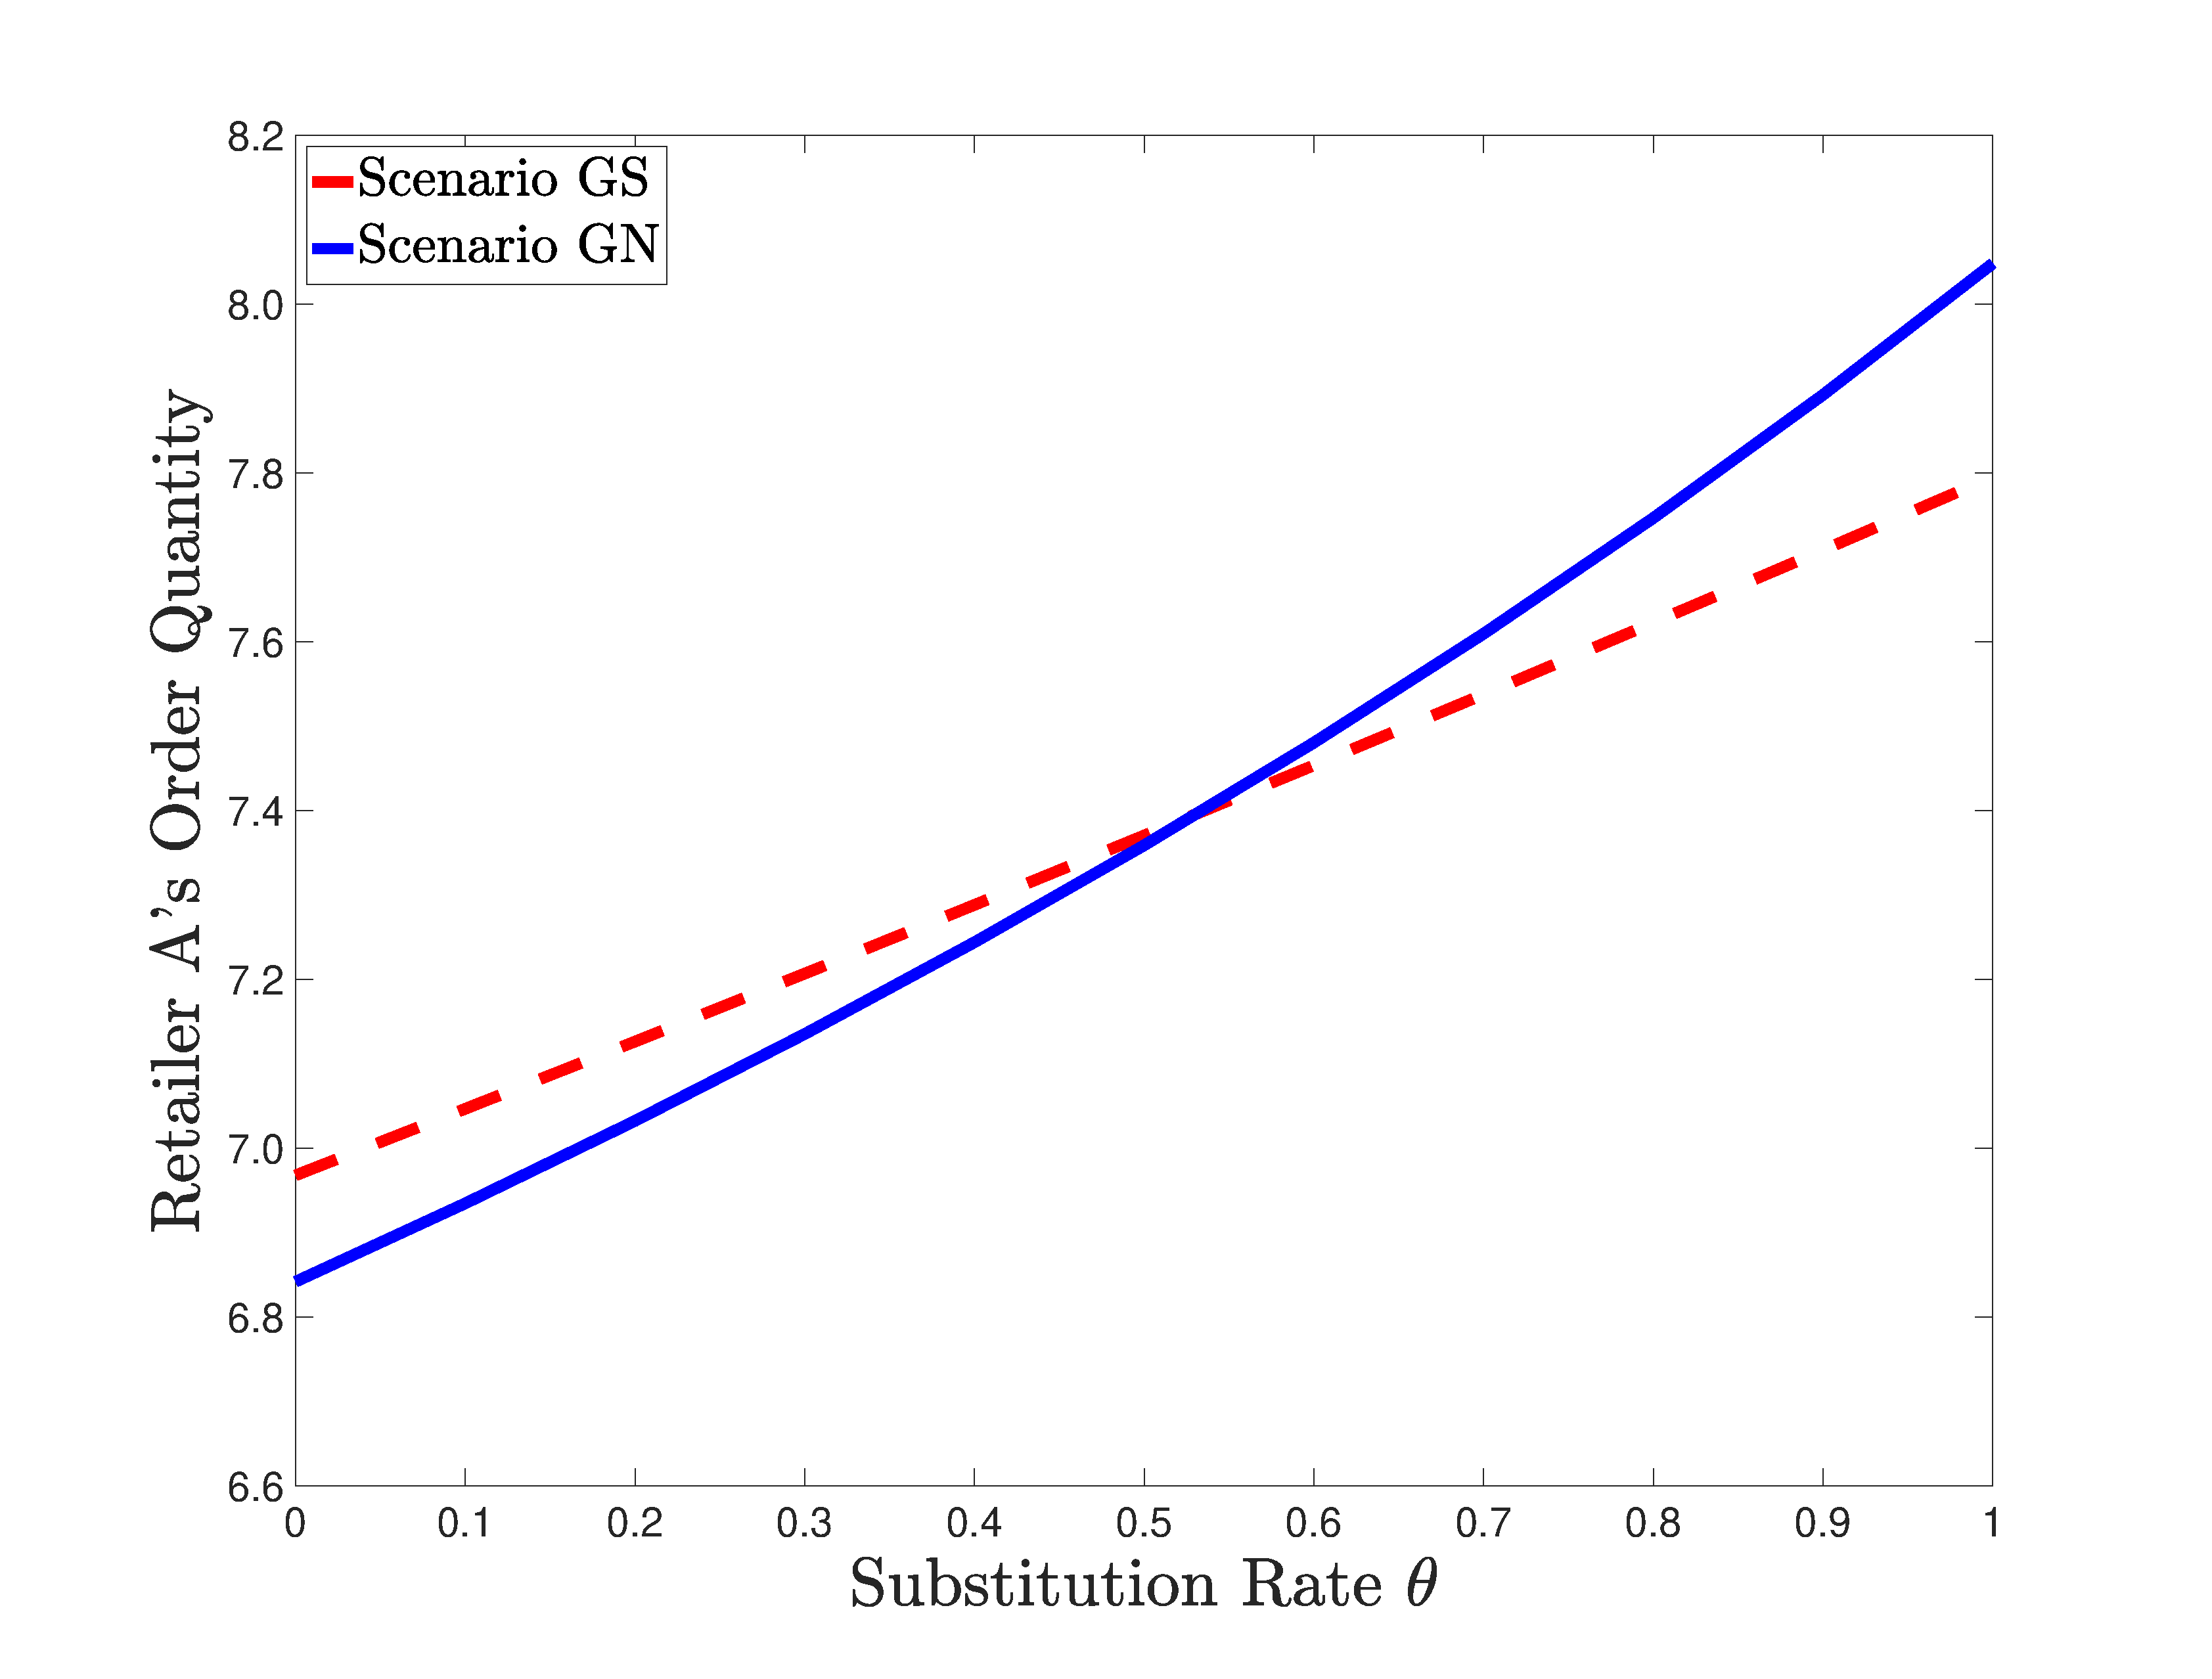
\includegraphics[width=\linewidth]{yaG.eps}
  \caption{Retailer A's order quantity; $c_A = 0.5$}
  \label{fig:general-ya}
\end{subfigure}
\begin{subfigure}{.45\linewidth}
  \centering
  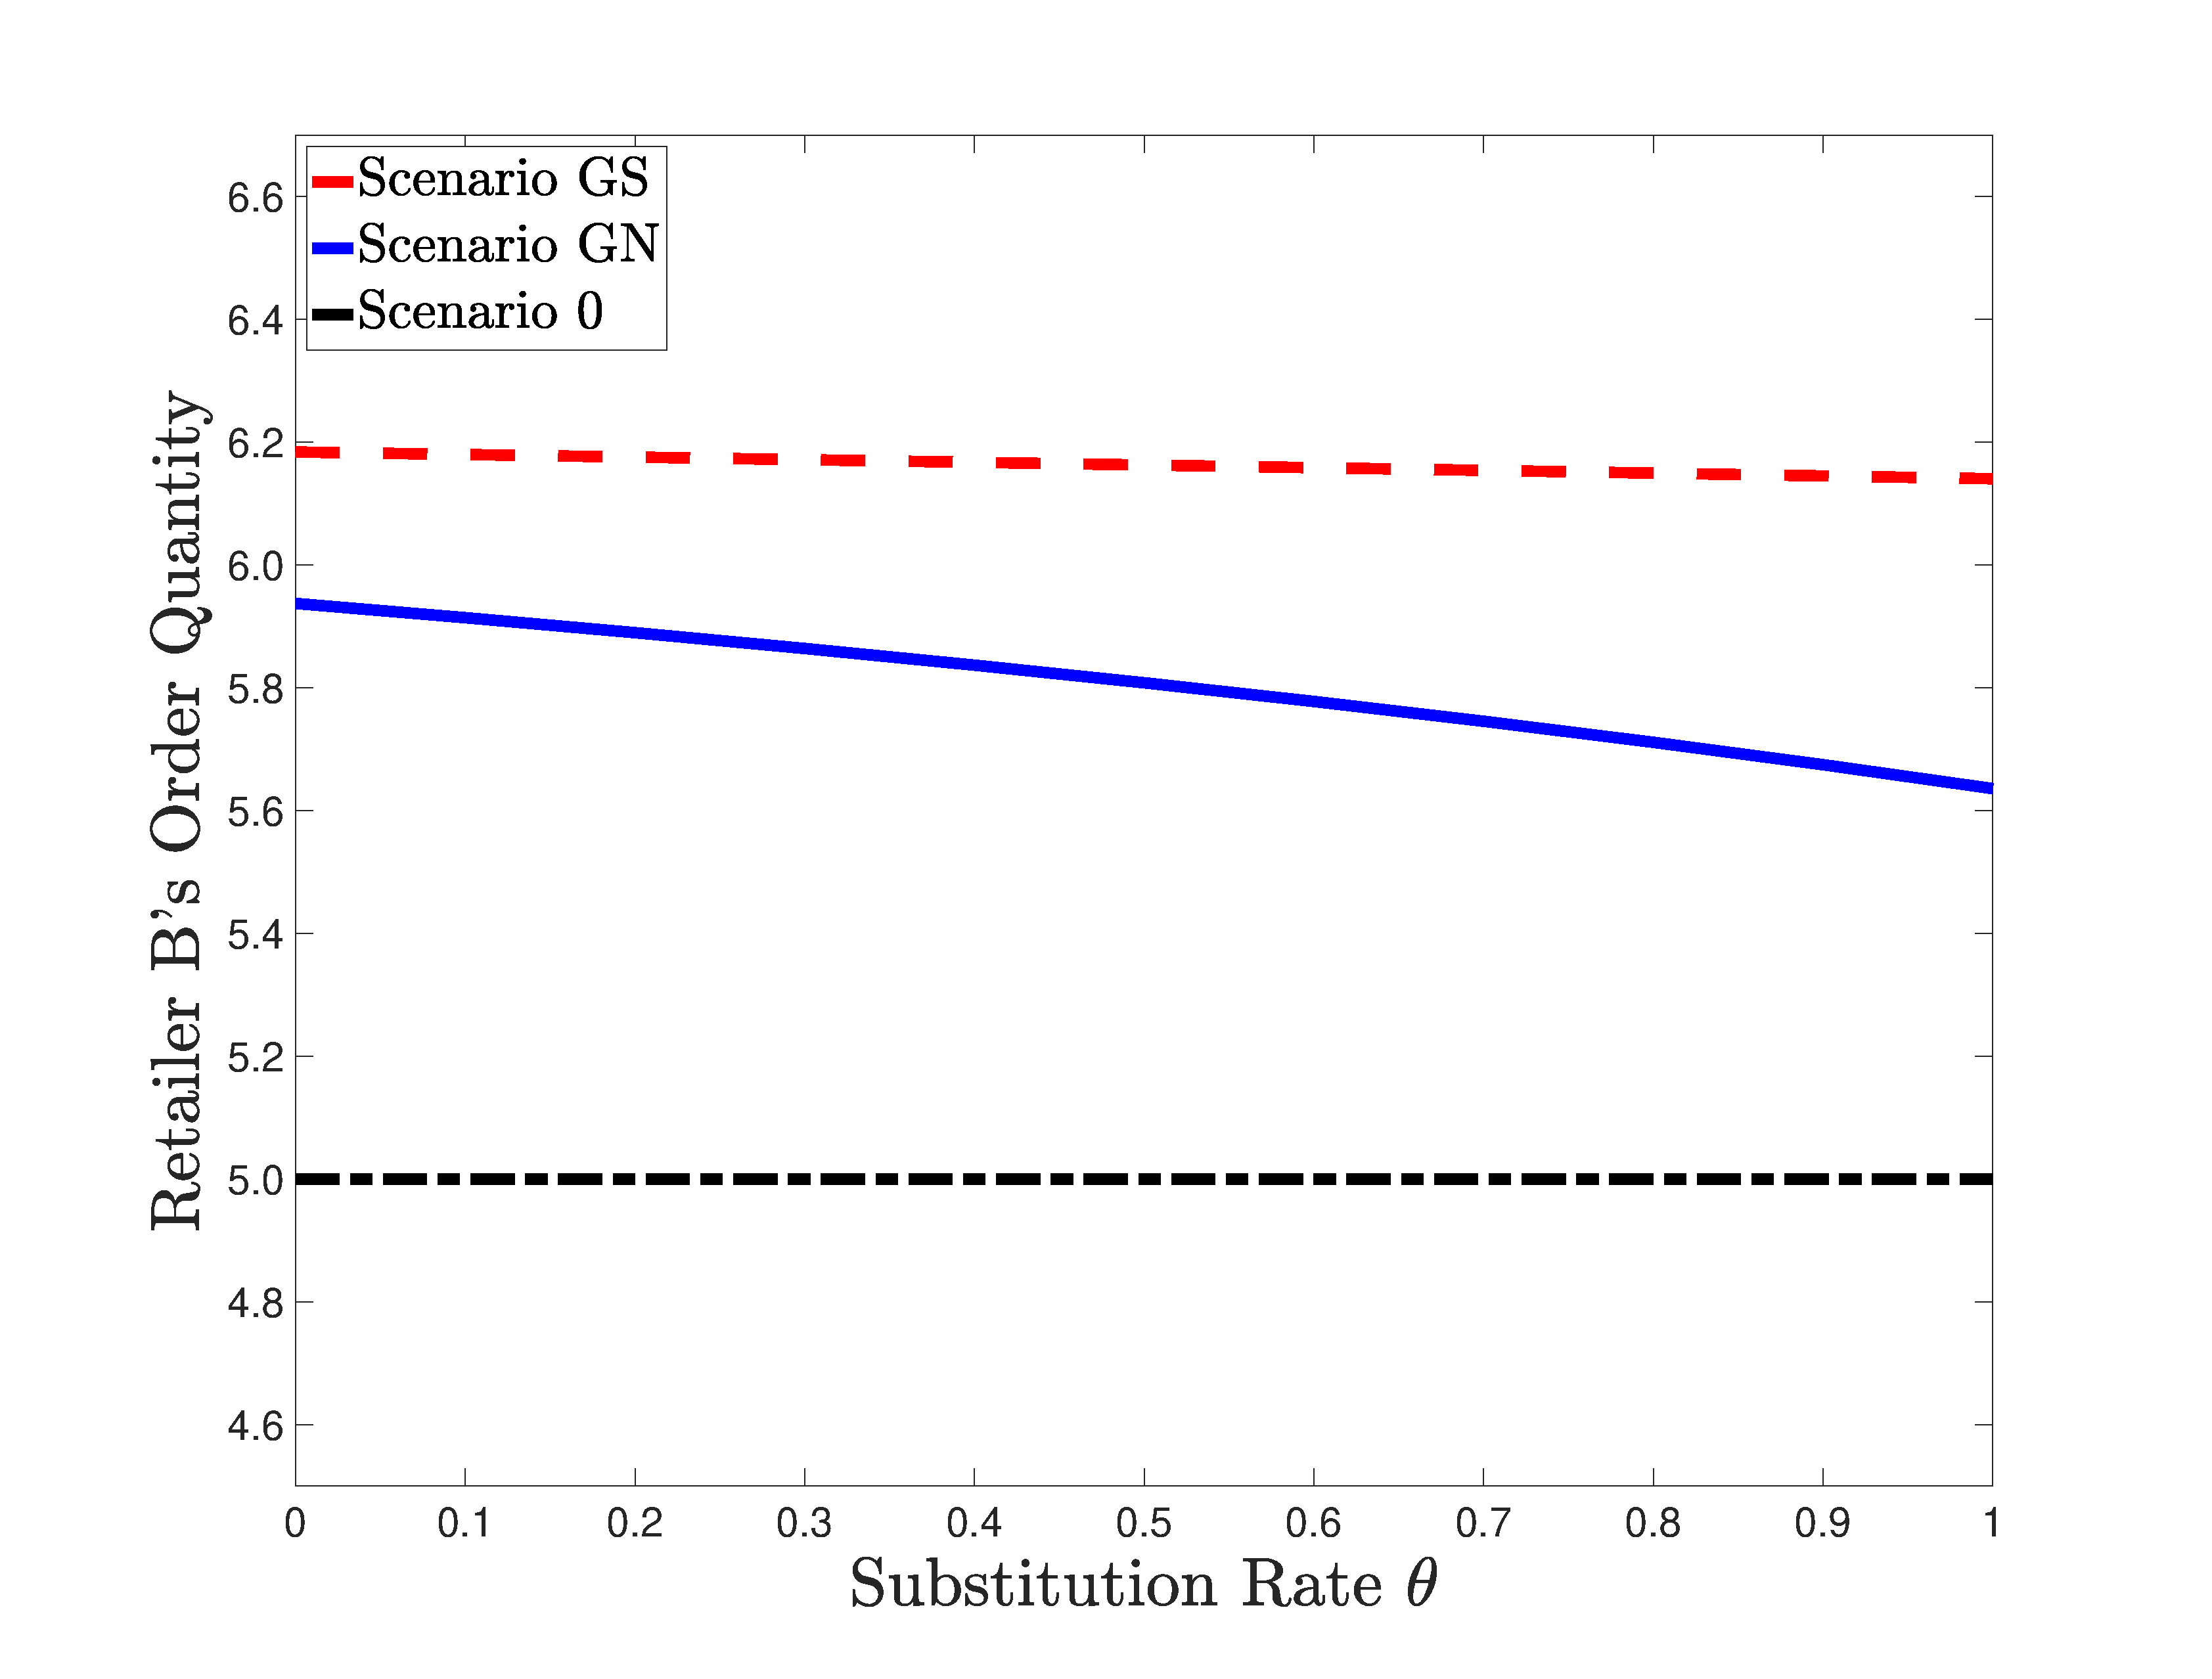
\includegraphics[width=\linewidth]{ybG.eps}
  \caption{Retailer B's order quantity; $c_A = 0.5$}
  \label{fig:general-yb}
\end{subfigure}
\\
\begin{subfigure}{.45\linewidth}
  \centering
  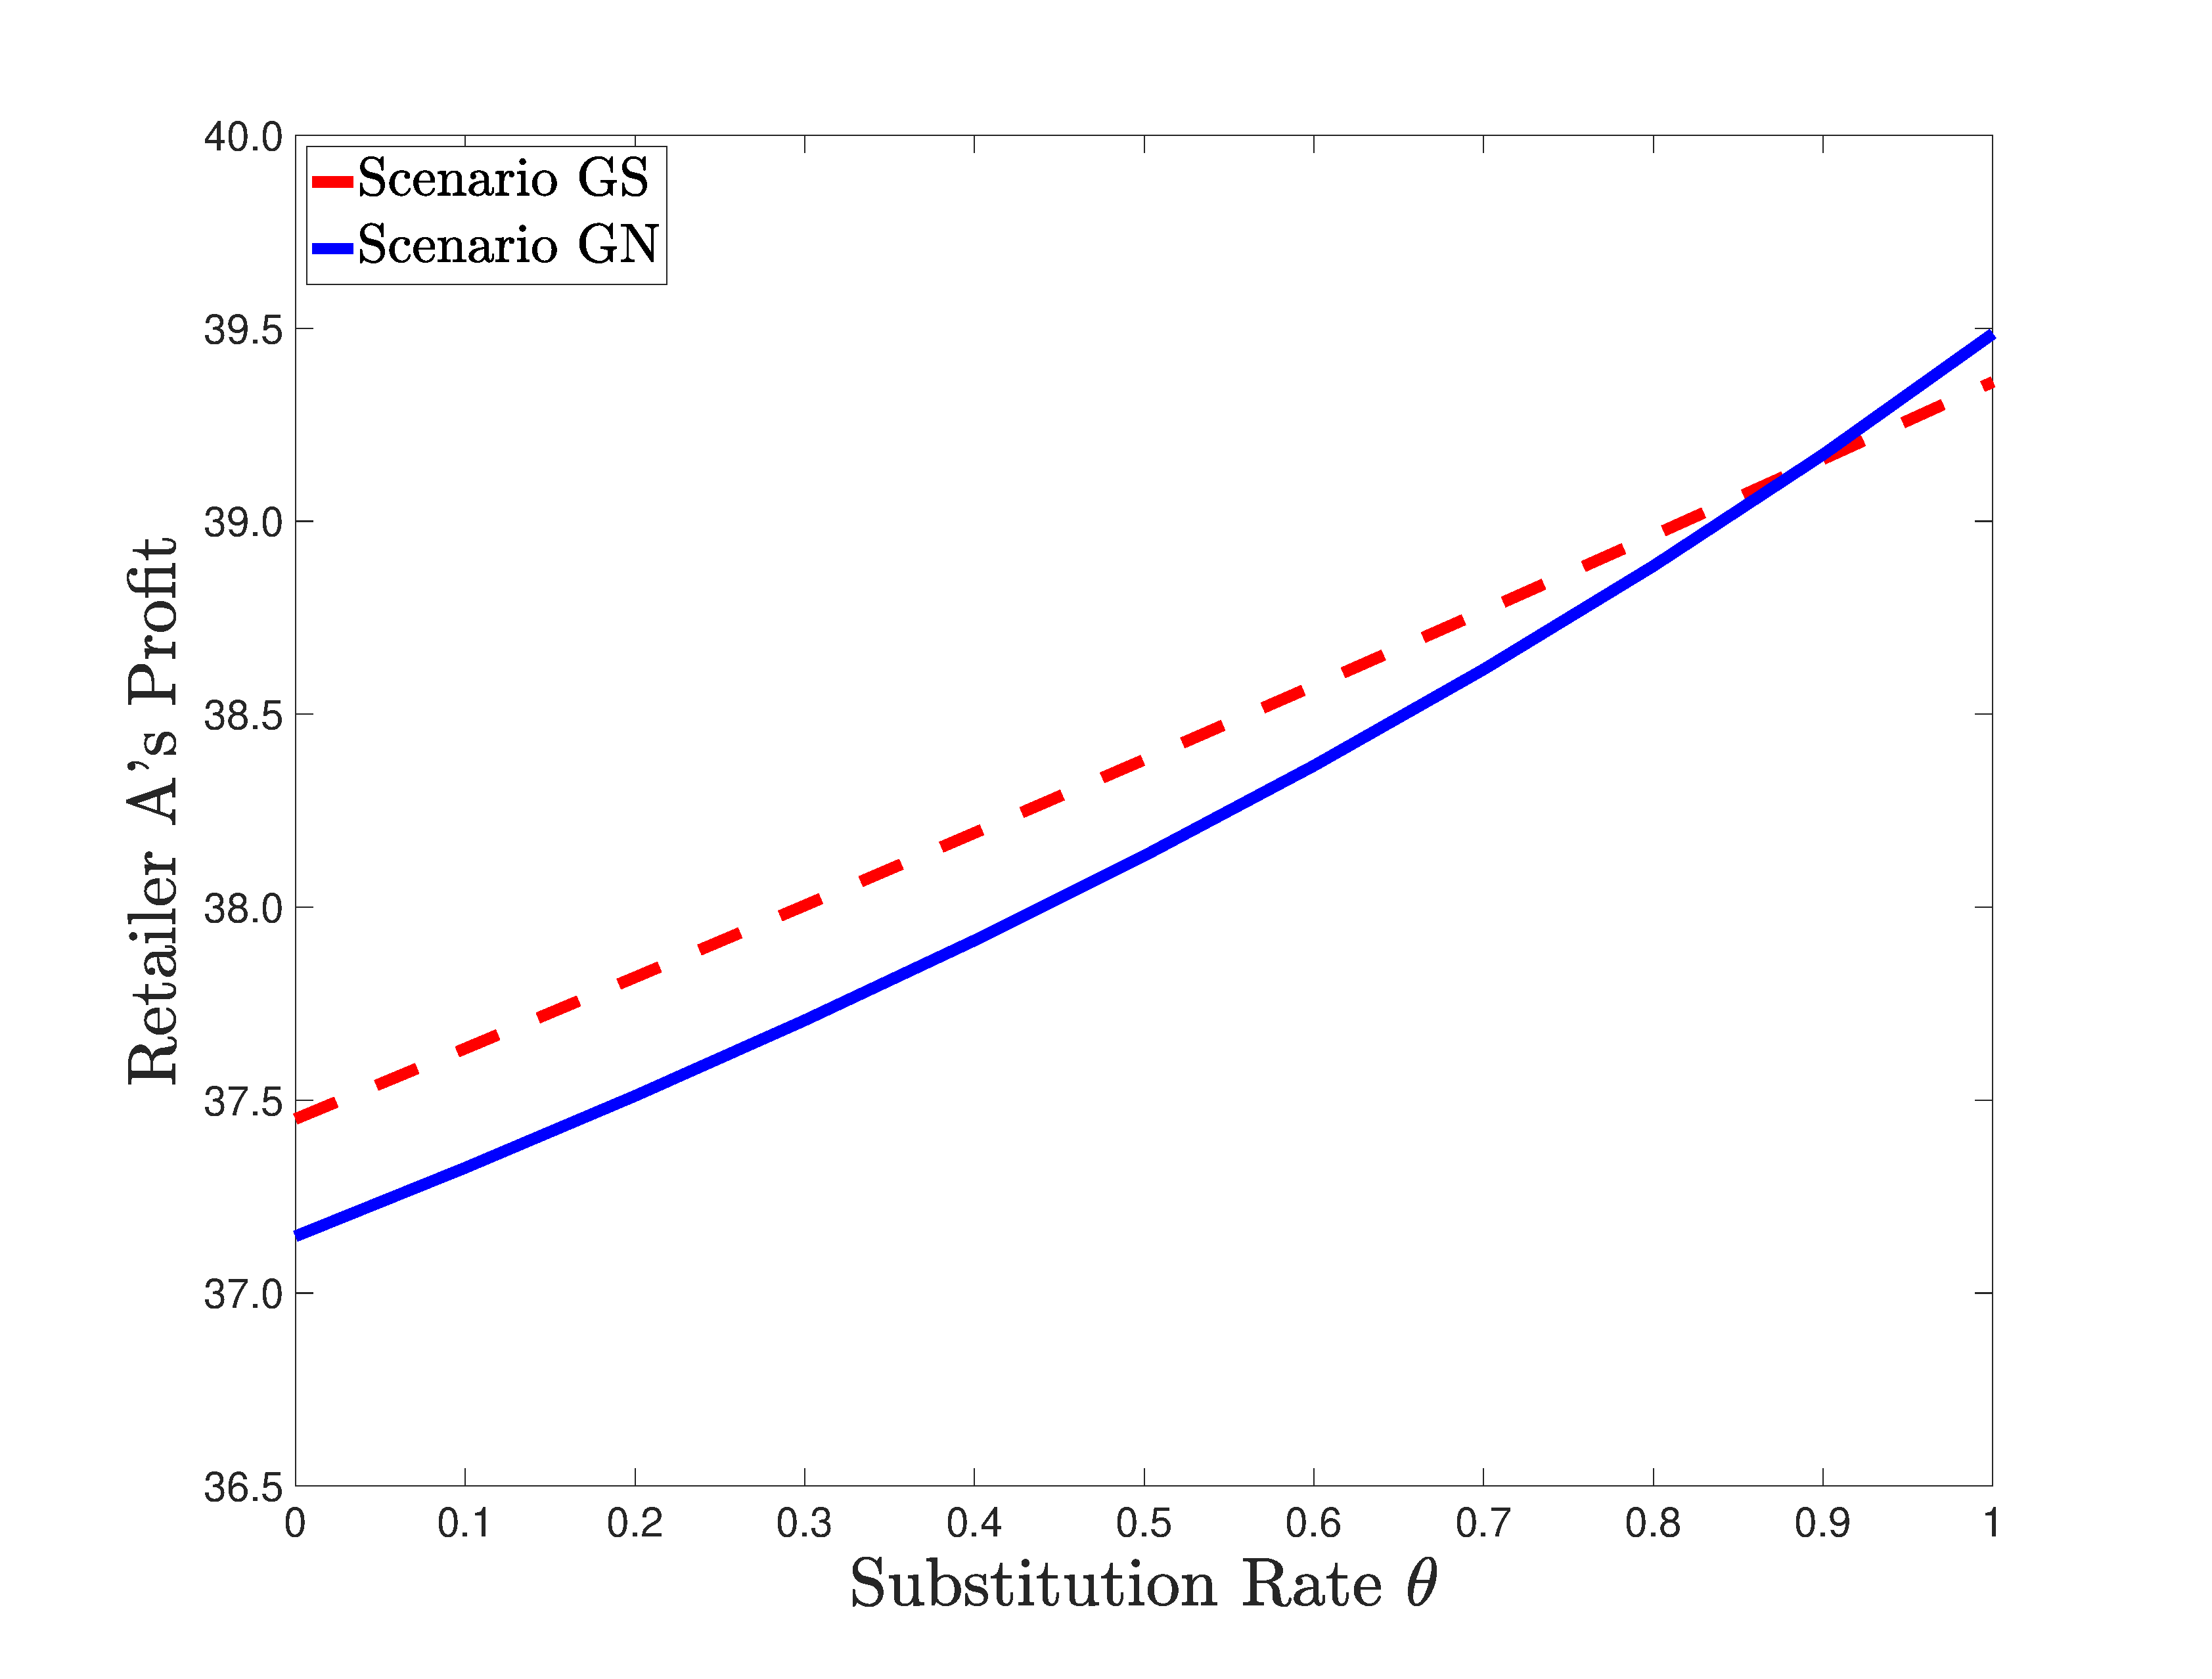
\includegraphics[width=\linewidth]{piaG.eps}
  \caption{Retailer A's profit comparison; $c_A = 0.1$}
  \label{fig:general-pfta}
\end{subfigure}
\begin{subfigure}{.45\linewidth}
  \centering
  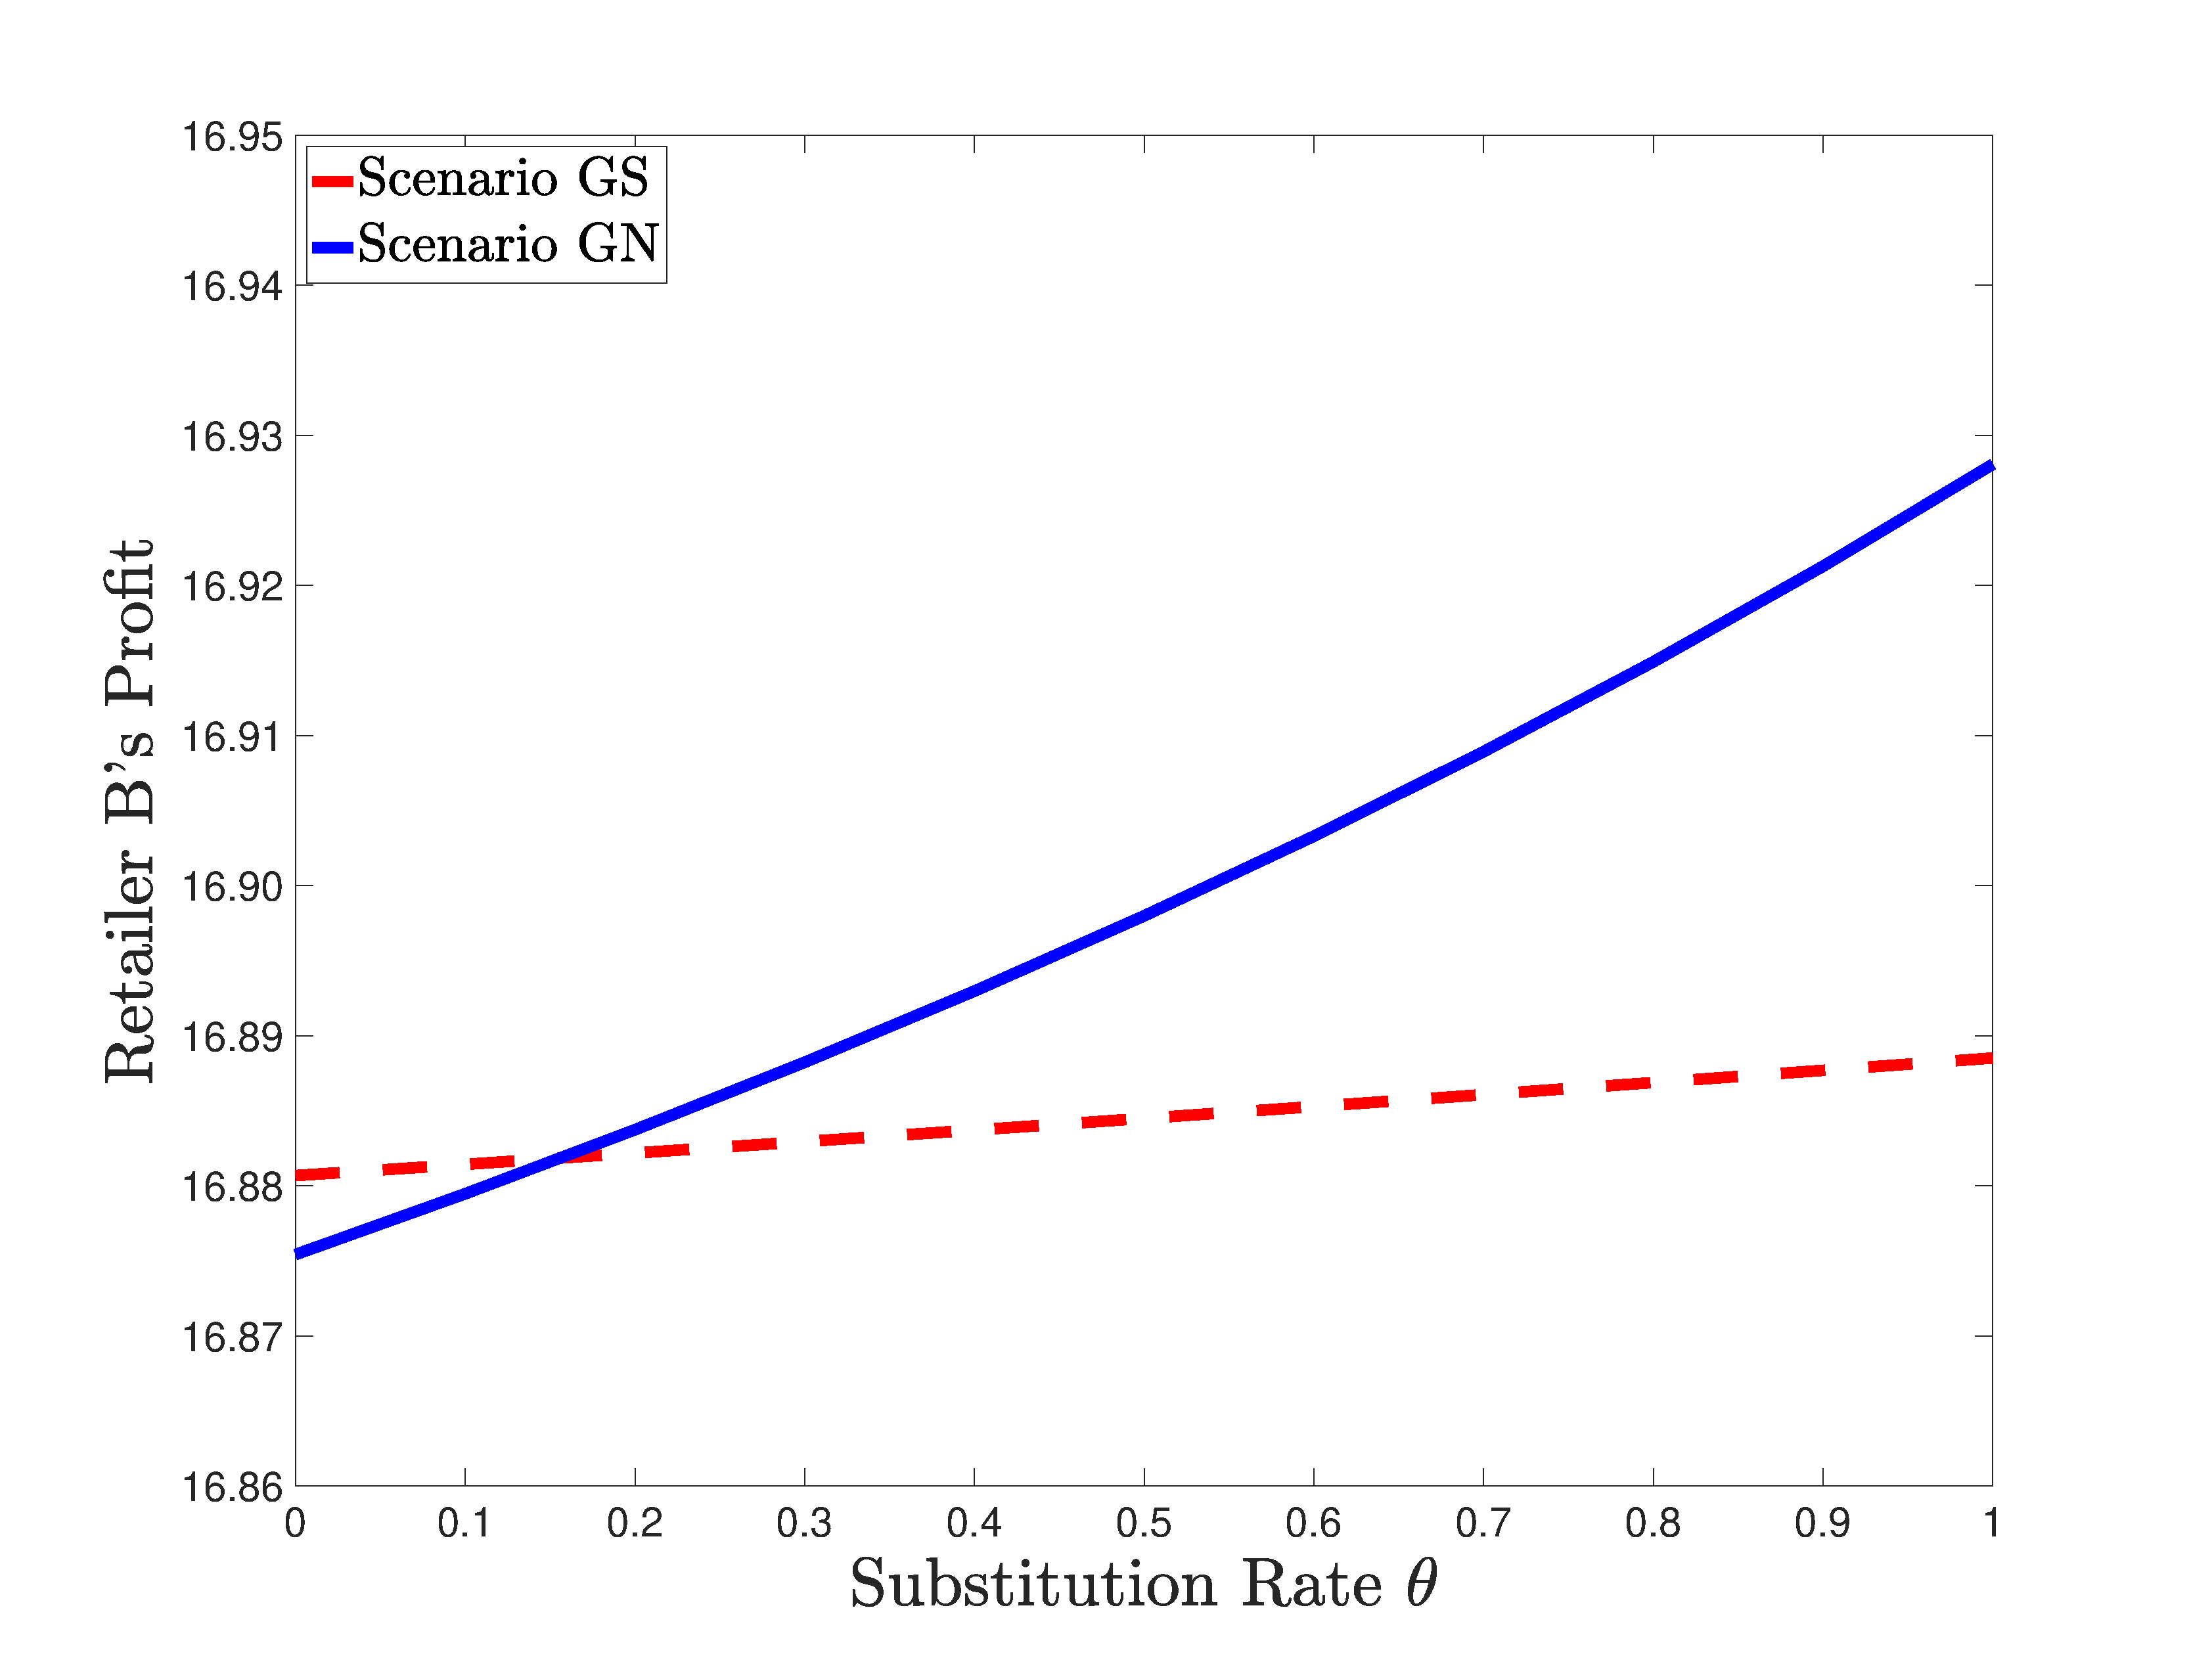
\includegraphics[width=\linewidth]{pibG.eps}
  \caption{Retailer B's profit comparison; $c_A= 0.92$}
  \label{fig:general-pftb}
\end{subfigure}

\begin{flushleft}
    {\footnotesize \emph{Parameters:} We fix $p_{i,t} = 2 (i = A, B; t = 1, 2)$, $c_B=1$, $\beta=0.1$, $X_t \sim U[5,15] (t = 1, 2)$. For Scenario GS, we choose $\gamma = 2$,  $\lambda^S = 0.8$, and $\lambda^N = 0.2$; and for Scenario GN, we choose $\gamma = 2$, $\lambda^S = 0.2$, and $\lambda^N = 0.8$. For the benchmark (Scenario $0$), we choose $\gamma = 0$.}
\end{flushleft}
\end{figure}

\end{APPENDICES}
\end{document}
